%%%%%%%%%%%%%%%%%%%%%%%%%%%%%%%%%%%%%%%%%%%%%%%%%%%%%%%%%%%%%%%%%%%%%%%%%%%%%
%%                                                                         %%
%%                   LaTeX Vorlage für die Studenten der                   %%
%%              Dualen Hochschule Baden-Württemberg Ravensburg             %%
%%                                                                         %%
%%  Die Vorlage orientiert sich an den Gestaltungsrichtlinien der DHBW RV  %%
%%                                                                         %%
%%                                                                         %%
%% Ersteller:        Markus Schutz (WI06)                                  %%
%% letzten Änderung: 26. November 2013                                     %%
%%                                                                         %%
%%                                                                         %%
%% Wichtiger Hinweis zur Verwendung dieser Vorlage:                        %%
%%                                                                         %%
%% Damit die Vorlage verwendet und die PDF richtig und vollständig erzeugt %%
%% werden kann bedarf des manuellen Aufrufs von makeindex. Diese können    %%
%% optional auch direkt im Editor eingerichtet werden.                     %%
%% TeXnicCenter (Ausgabe -> Ausgabeprofile definieren... (Alt + F7)        %%
%%               LaTeX => PDF -> Nachbearbeitung)                          %%
%%                                                                         %%
%% (1) Stichwortverzeichnis (falls verwendet)                              %%
%% makeindex -g -s styles\stichwortverzeichnis.ist vorlage                 %%
%% (2) Abkürzungsverzeichnis                                               %%
%% makeindex vorlage.nlo -s cl.ist -o vorlage.nls                     %%
%% (3) Glossar (falls verwendet)                                           %%
%% makeindex -s vorlage.ist -t vorlage.glg -o vorlage.gls vorlage.glo      %%
%%                                                                         %%
%% Bei der Erzeugung der PDF Datei (Anwendung des LaTeX => PDF Ausgabe-    %%
%% profiles) werden das Abkürzungsverzeichnis, das Stichwortverzeichnis    %%
%% und das Glossar jetzt richtig erzeugt. In Verbindung mit TeXnicCenter   %%
%% kann es beim automatisierten Aufruf von makeindex zu Probleme kommen.   %%
%% Ein manueller Aufruf funktioniert dagegen immer.                        %%
%%                                                                         %%
%% Wichtiger Hinweis:                                                      %%
%%                                                                         %%
%% Keine Änderungen an den Dateien im Verzeichnis "pages" vornehmen. Für   %%
%% die Arbeit beziehen sich alle Änderungen auf diese Datei und die        %%
%% Dateien im Verzeichnis "chapter".                                       %%
%% Für die Erstellung des Literaturverzeichnises empfiehlt sich die Ver-   %%
%% wendung von JabRef (http://jabref.sourceforge.net). Die Datei ist unter %%
%% dem Namen literatur.bib im Verzeichnis "literatur" zu speichern.        %%
%%                                                                         %%
%% Zur sinnvollen Nutzung dieser Vorlage empfiehlt es sich, die Dokus zu   %%
%% den eingebundenen Paketen durchzulesen. Sie sind im doc-Verzeichnis der %%
%% MiKTeX-Installation zu finden.                                          %%
%%                                                                         %%
%% Enthaltene Titelblätter:                                                %%
%%   - Seminararbeit                                                       %%
%%   - Projektarbeit                                                       %%
%%   - Bachelorarbeit                                                      %%
%%                                                                         %%
%%%%%%%%%%%%%%%%%%%%%%%%%%%%%%%%%%%%%%%%%%%%%%%%%%%%%%%%%%%%%%%%%%%%%%%%%%%%%

\documentclass[a4paper,12pt]{article}                                         % Schriftgröße, Layout, Papierformat, Art des Dokumentes
\usepackage[left=3cm,right=2cm,top=2cm,bottom=2cm,includehead]{geometry}      % Einstellungen der Seitenränder
\usepackage{ngerman}                                                          % neue Rechtschreibung
\usepackage[main=ngerman,english]{babel} 
\usepackage{lmodern}                                                  % deutsche Silbentrennung
\usepackage[utf8]{inputenc} 
%\usepackage[ansinew]{inputenc}                                                  % Umlaute
\usepackage[T1]{fontenc}
\usepackage{textcomp}
\usepackage[hyperfootnotes=false]{hyperref}                                   % pfd-Output [Fußnoten nicht verlinken]
\usepackage[nottoc]{tocbibind}                                                % Inhaltsverzeichniserweiterung (Inhaltsverzeichnis selbst ausblenden)
\usepackage{makeidx}                                                          % Index
\usepackage[intoc]{nomencl}                                                   % Abkürzungsverzeichnis
\usepackage{fancyhdr}                                                         % Fancy Header
\usepackage[round]{natbib}                                                    % Zitate (Erweiterung für Literaturverzeichnis)
\usepackage{amsmath}                                                          % Zurücksetzen der Tabellen- und Abbildungsnummerierung je Sektion
\usepackage[labelfont=bf,aboveskip=1mm]{caption}                              % Bild- und Tabellenunterschrift (fett)
\usepackage{setspace}                                                         % Zeilenabstand (vor footmisc laden!)
\usepackage[bottom,multiple,hang,marginal]{footmisc}                          % Fußnoten [Ausrichtung unten, Trennung durch Seperator bei mehreren Fußnoten]
\usepackage{graphicx}                                                         % Grafiken
\usepackage{tabularx}                                                         % erweiterte Tabellen
\usepackage{longtable}                                                        % mehrseitige Tabellen
\usepackage{color}                                                            % Farben
\usepackage{enumitem}                                                         % Befehl setlist (Zeilenabstand für itemize Umgebung auf 1 setzen)
\usepackage[formats]{listings}                                                         % Quelltexte
\usepackage{zref}                                                             % Verweise (Anhangsverweise)
\usepackage[toc,style=altlist,translate=false]{glossaries}                    % Glossar (nach hyperref, 
%\usepackage{glossaries-babel}                                                 % Glossar: Übersetzung im TOC
\usepackage{url}
\usepackage[autostyle]{csquotes}
\usepackage{framed}
\usepackage{lipsum}
\usepackage[final]{pdfpages}
\usepackage{float}															% Platzierung der Bilder
\definecolor{shadecolor}{gray}{0.9}
\definecolor{gray}{rgb}{0.4,0.4,0.4}
\definecolor{darkblue}{rgb}{0.0,0.0,0.6}
\definecolor{cyan}{rgb}{0.0,0.6,0.6}




%%%%%%%%%%%%%%%%%%%%%%%%%%%%%%%%%%%%%%%%%%%%%%%%%%%%%%%%%%%%%%%%%%%%%%%%%%%%%
%%                                                                         %%
%% \/   \/      Bitte hier die Änderungen zur Arbeit vornehmen     \/   \/ %%
%%                                                                         %%
%%%%%%%%%%%%%%%%%%%%%%%%%%%%%%%%%%%%%%%%%%%%%%%%%%%%%%%%%%%%%%%%%%%%%%%%%%%%%

%%%%%%%%%%%%%%%%%%%%%%% Definitionen bzgl. der Arbeit %%%%%%%%%%%%%%%%%%%%%%%
\def\myType{3}           % [0=Seminararbeit|1=Projektarbeit|2=Bachelorarbeit|3=Studienarbeit]

\def\myTopic{Prototypische Implementierung eines Dozentenfinders mittels Bluetooth-Technologie}
\def\mySubTopic{ zur Machbarkeits-Evaluierung des “DeSearch”-Projekts }
\def\myAutor{Philipp Stehle und Lina Hirschoff}
\def\myMatNr{5316233 und 4125931}
\def\myCompany{SAP SE}
\def\myCompanyAddressStreet{Dornierstraße 3}
\def\myCompanyAddressCity{88677 Markdorf}
\def\myProf{Andreas Judt}
\def\myEndDate{15.07.2016}
\def\myEditDate{KW 40/2015 - KW 28/2016}

%%%%%%%%%%%%%%%%%%%% Folgende Angaben für: Seminararbeit %%%%%%%%%%%%%%%%%%%%
\def\myVorlesung{Name der Vorlesung}

%%%%%%%%%%%%%%%%%%%% Folgende Angaben für: Projektarbeit %%%%%%%%%%%%%%%%%%%%
\def\myProjNumber{4}         % [1|2]
\def\myPraxPhase{3}                       % [1|2|3]

%%%%%%%%%%%%%%%%%%%%%%%%%%%%%%%%%%%%%%%%%%%%%%%%%%%%%%%%%%%%%%%%%%%%%%%%%%%%%
%%                                                                         %%
%% /\   /\         Ab hier keine Änderungen mehr vornehmen         /\   /\ %%
%%                                                                         %%
%%%%%%%%%%%%%%%%%%%%%%%%%%%%%%%%%%%%%%%%%%%%%%%%%%%%%%%%%%%%%%%%%%%%%%%%%%%%%

%%%%%%%%%%%%%%%%%%%%%%%% Eigene Farbwerte definieren %%%%%%%%%%%%%%%%%%%%%%%%
\definecolor{boxgray}{gray}{0.9}         % Hintergrundfarbe für Zitatboxen
\definecolor{commentgray}{gray}{0.5}     % Grau für Kommentare in Quelltexten
\definecolor{darkgreen}{rgb}{0,.5,0}     % Grün für Strings in Quelltexten
\definecolor{purple}{rgb}{0.44, 0.16, 0.39} %Lila für JS-Keywords in Quelltexten


%%%%%%%%%%%%%%%%%%%%%%%% Eigene Kommandos definieren %%%%%%%%%%%%%%%%%%%%%%%%
% Definition von \gqq{#1: text}: Text in Anführungszeichen
\newcommand{\gqq}[1]{\glqq #1\grqq}

% Definition von \footref{#1: label}
% Verweis auf bereits existierende Fußnoten mittels
\providecommand*{\footref}[1]{
	\begingroup
		\unrestored@protected@xdef\@thefnmark{\ref{#1}}
	\endgroup
\@footnotemark}

% Definition von \mypageref{#1: label}
% Kombination aus \ref{#1: label} und \pageref{#1: label}
\newcommand{\mypageref}[1]{\ref{#1} auf Seite \pageref{#1}}

% Definition von \myboxquote{#1: text}
% grau hinterlegte Quotation-Umgebung (für Zitate)
\newcommand{\myboxquote}[1]{
	\begin{quotation}
		\colorbox{boxgray}{\parbox{0.78\textwidth}{#1}}
	\end{quotation}
	\vspace*{1mm}
}

\makeatletter
\zref@newprop*{appsec}{}
\zref@addprop{main}{appsec}

% Definition von \applabel{#1: label}{#2: text}
% von \appsec{#1: text}{#2: label} zur Erzeugung des Labels verwendet)
\def\applabel#1#2{%
	\zref@setcurrent{appsec}{#2}%   
	\zref@wrapper@immediate{\zref@label{#1}}%
}

% Definition von \appref{#1: label}
% anstelle \ref{#1: label} zum referenzieren von Anhängen verwenden)
\def\appref#1{%
	\hyperref[#1]{\zref@extract{#1}{appsec}}%
}
\makeatother

% Definition von \appsection{#1: text}{#2: label}
% Ersetzt \section{#1: text} und \label{#2: label} für Anhänge)
\newcommand{\theappsection}[1]{Anhang \Alph{section}:~\protect #1}
\newcommand{\appsection}[2]{
	\addtocounter{section}{1}
	\phantomsection
	\addcontentsline{toc}{section}{\theappsection{#1}}
	\markboth{\theappsection{#1}}{}

	\section*{\theappsection{#1}}
	\applabel{#2}{Anhang \Alph{section}}
	\label{#2}
}

\newcommand\tab[1][1cm]{\hspace*{#1}}

%%%%%%%%%%%%% Index, Abkürzungsverzeichnis und Glossar erstellen %%%%%%%%%%%%
\makeindex
\makenomenclature
\makeglossaries

% Festlegung der Art der Zitierung (Havardmethode: Abkuerzung Autor + Jahr) %
\bibliographystyle{dinat}

%%%%%%%%%%%%%%%%%%%%%%%%%%%%%%% PDF-Optionen %%%%%%%%%%%%%%%%%%%%%%%%%%%%%%%%
\hypersetup{
	bookmarksopen=false,
	bookmarksnumbered=true,
	bookmarksopenlevel=0,
	pdftitle=\myTopic,
	pdfsubject=\myTopic,
	pdfauthor=\myAutor,
	pdfborder=0 0 0,
	pdfstartview=Fit,
	pdfpagelayout=SinglePage
}

%%%%%%%%%%%%%%%%%%%%%%%%%%%% Kopf- und Fußzeile %%%%%%%%%%%%%%%%%%%%%%%%%%%%%
\pagestyle{fancy}
\fancyhf{}
\fancyhead[R]{\thepage}                         % Kopfzeile rechts bzw. außen
\renewcommand{\headrulewidth}{0.5pt}            % Kopfzeile rechts bzw. außen

%%%%%%%%%%%%%%%%%%%%%%%%% Layout und Beschriftungen %%%%%%%%%%%%%%%%%%%%%%%%%
\onehalfspacing                % Zeilenabstand: 1.5 (Standard: 1.2)
\setlist{noitemsep}            % Zeilenabstand für items auf 1 setzen

\addto\captionsngerman{        % Tabllen- und Abbildungsunterschriften ändern
  \renewcommand{\figurename}{Abb.}
  \renewcommand{\tablename}{Tab.}
}
\numberwithin{table}{section}                               % Tabellennummerierung je Sektion zurücksetzen
\numberwithin{figure}{section}                              % Abbildungsnummerierung je Sektion zurücksetzen
\renewcommand{\thetable}{\arabic{section}.\arabic{table}}   % Tabellennummerierung mit Section
\renewcommand{\thefigure}{\arabic{section}.\arabic{figure}} % Abbildungsnummerierung mit Section
\renewcommand{\thefootnote}{\arabic{footnote}}              % Sektionsbezeichnung von Fußnoten entfernen

\renewcommand{\multfootsep}{, }                             % Mehrere Fußnoten durch ", " trennen

%%%%%%%%%%%%%%%%%%%%%%%%%%%%%%% Listingstyle %%%%%%%%%%%%%%%%%%%%%%%%%%%%%%%%
\lstset{
%	basicstyle=\ttfamily\small
%	basicstyle=\scriptsize\ttfamily\bfseries,
%	basicstyle=\fontfamily{pcr}\selectfont\scriptsize,
	%basicstyle=\itshape\small,
 basicstyle=\footnotesize\ttfamily,
	commentstyle=\color{commentgray}\textit,
	showstringspaces=false,
	stringstyle=\color{darkgreen},
	keywordstyle=\color{blue},
%	numbers=left,
%	numberstyle=\tiny,
%	stepnumber=1,
%	numbersep=10pt,
	tabsize=2,
	showspaces=false,
	keepspaces=true
	showtabs=false,
	fontadjust=true,
	frame=single,
%	backgroundcolor=\color{boxgray},
	captionpos=b,
	linewidth=1.0\linewidth,
	xleftmargin=0\linewidth,
	breaklines=true,
	aboveskip=16pt
}
\lstdefinelanguage{XML}
{
  morestring=[b]",
  morestring=[s]{>}{<},
  morecomment=[s]{<?}{?>},
  stringstyle=\color{black},
  identifierstyle=\color{darkblue},
  keywordstyle=\color{cyan},
  morekeywords={xmlns,version,type}% list your attributes here
}
\lstdefinelanguage{JavaScript}{
  keywords={break, case, catch, continue, debugger, default, delete, do, else, false, finally, for, function, if, in, instanceof, new, null, return, switch, this, throw, true, try, typeof, var, void, while, with},
  morecomment=[l]{//},
  morecomment=[s]{/*}{*/},
  morestring=[b]',
  morestring=[b]",
  ndkeywords={class, export, boolean, throw, implements, import, this},
  keywordstyle=\color{blue}\bfseries,
  ndkeywordstyle=\color{darkgray}\bfseries,
  identifierstyle=\color{black},
  commentstyle=\color{purple}\ttfamily,
  stringstyle=\color{darkgreen}\ttfamily,
  sensitive=true
}

        
%%%%%%%%%%%%%%%%%%%%%%%%%%%%%%%%%%%%%%%%%%%%%%%%%%%%%%%%%%%%%%%%%%%%%%%%%%%%%
%%                                                                         %%
%% \/   \/      Bitte hier die Änderungen zur Arbeit vornehmen     \/   \/ %%
%%                                                                         %%
%%%%%%%%%%%%%%%%%%%%%%%%%%%%%%%%%%%%%%%%%%%%%%%%%%%%%%%%%%%%%%%%%%%%%%%%%%%%%

%Seiten und Kapitel einbinden
\begin{document}
	\pagenumbering{Roman}
	% Das Titelblatt wird automatisch ausgewählt. Keine Änderung hier
	\ifcase\myType
		\begin{titlepage}
	\begin{center}
		\vspace*{2cm}
		\LARGE\bf\myTopic\\
		\Large\rm\mySubTopic\\
		\vspace*{3cm}
		\bf Seminararbeit zur Vorlesung\\
		\myVorlesung\\
		\normalsize\rm
		\vspace*{1cm}
		für die\\
		Prüfung zum Bachelor of Engineering\\
		\vspace*{1cm}
		an der Fakultät für Technik\\
		im Studiengang Informationstechnik\\
		\vspace*{1cm}
		an der\\
		DHBW Ravensburg\\
		Campus Friedrichshafen
		\vfill
	\end{center}
	\begin{tabular}{ll}
		Verfasser:&\myAutor\\
		Ausbildungsbetrieb:&\myCompany\\
		Anschrift:&\myCompanyAddressStreet\\
		&\myCompanyAddressCity\\
	%	Wiss. Betreuer:&\myProf\\
		Abgabedatum:&\myEndDate\\
	\end{tabular}
\end{titlepage}
\newpage
\setcounter{page}{2}

	\or
		\begin{titlepage}

\begin{table}
\begin{tabular}{p{0.4\textwidth}p{0.4\textwidth}}
\includegraphics[width=4cm]{images/sap_logo.png} &
\hfill 
\includegraphics[width=4cm]{images/dhbw_logo.jpg} \\
\end{tabular}
\end{table}

	\begin{center}
		\vspace*{1cm}
		\LARGE\bf\myTopic\\
		%\Large\rm\mySubTopic\\
		\vspace*{1cm}
		\bf Projektarbeit\\
		
		\normalsize\rm
		 im \myPraxPhase. Studienjahr \\
		\vspace*{1cm}
		
		Duale Hochschule Baden-Württemberg\\
		\vspace*{0.5cm}
		TIT13 Informationstechnik\\
		\vspace*{1cm}
		von\\
		 \myAutor\\
		\vspace*{1cm}
		
		\vfill
	\end{center}
	\begin{tabular}{ll}
		Abgabe:&\myEndDate\\
		Bearbeitungszeitraum:&\myEditDate\\
		Matrikelnummber:&\myMatNr\\
		Partnerunternehmen:&\myCompany\\
		Addresse:&\myCompanyAddressStreet\\
					&\myCompanyAddressCity\\
		\\
		Betreuer:&\myProf\\
		
	\end{tabular}
	\newline
	\vspace*{1cm}
%	\newline
%	\begin{tabularx}{\textwidth}{l@{\extracolsep\fill}r}
%	  Unterschrift des verantwortlichen Ausbilders&\\
%	  (oder des Personalverantwortlichen)&\rule{6cm}{0.3mm}\\
%	\end{tabularx}
\end{titlepage}
\newpage
\setcounter{page}{2}

	\or
		\begin{titlepage}
	\begin{center}
		\vspace*{2cm}
		\LARGE\bf\myTopic\\
		\Large\rm\mySubTopic\\
		\vspace*{3cm}
		\bf Bachelorarbeit\\
		\normalsize\rm
		\vspace*{1cm}
		für die\\
		Prüfung zum Bachelor of Science\\
		\vspace*{1cm}
		an der Fakultät für Wirtschaft\\
		im Studiengang Wirtschaftsinformatik\\
		\vspace*{1cm}
		an der\\
		DHBW Ravensburg
		\vfill
	\end{center}
	\begin{tabular}{ll}
		Verfasser:&\myAutor\\
		Ausbildungsbetrieb:&\myCompany\\
		Anschrift:&\myCompanyAddressStreet\\
		&\myCompanyAddressCity\\
		Wiss. Betreuer:&\myProf\\
		Abgabedatum:&\myEndDate\\
	\end{tabular}
\end{titlepage}
\newpage
\setcounter{page}{2}

	\or
		\begin{titlepage}

\begin{table}
\begin{tabular}{p{0.4\textwidth}p{0.4\textwidth}}
%\includegraphics[width=4cm]{images/sap_logo.png} &
\hfill 
\includegraphics[width=6cm]{images/dhbw_logo.jpg} \\
\end{tabular}
\end{table}

	\begin{center}
		\vspace*{1cm}
		\LARGE\bf\myTopic\\
		\Large\rm\mySubTopic\\
		\vspace*{1cm}
		\bf Studienarbeit\\
		
		\normalsize\rm
		 im 3. Studienjahr \\
		\vspace*{1cm}
		
		Duale Hochschule Baden-Württemberg\\
		\vspace*{0.5cm}
		TIT13 Informationstechnik\\
		\vspace*{1cm}
		von\\
		 \myAutor\\
		\vspace*{1cm}
		
		\vfill
	\end{center}
	\begin{tabular}{ll}
		Abgabe:&\myEndDate\\
		Bearbeitungszeitraum:&\myEditDate\\
		Matrikelnummer:&\myMatNr\\
		
		Betreuer:&\myProf\\
		
	\end{tabular}
	\newline
	\vspace*{1cm}
%	\newline
%	\begin{tabularx}{\textwidth}{l@{\extracolsep\fill}r}
%	  Unterschrift des verantwortlichen Ausbilders&\\
%	  (oder des Personalverantwortlichen)&\rule{6cm}{0.3mm}\\
%	\end{tabularx}
\end{titlepage}
\newpage
\setcounter{page}{2}

	\else
	\fi
	
	\pagestyle{fancy}
	\thispagestyle{empty}
\addcontentsline{toc}{section}{Selbständigkeitserklärung}
\begin{center}
	\vspace*{2cm}
	\Huge\bf Selbständigkeitserklärung\\
	\vspace*{2cm}
	\normalsize\rm
	gemäß Ziffer 1.2.3 der Anlage 1 zu §§ 3, 4, und 5  der „Studien- und Prüfungsordnung DHBW Technik“ vom 29. September 2015.\\
	\vspace*{1cm}
	\normalsize\rm
	Ich versichere hiermit, dass ich meine \ifcase\myType Seminararbeit \or Projektarbeit \or Bachelorarbeit \or Studienarbeit \else\fi mit dem Thema: \\
	\vspace*{1cm}
	\Large\bf\myTopic\\
	\Large\rm\mySubTopic\\
	\vspace*{1cm}
	\normalsize\rm
	selbständig verfasst und keine anderen als die angegebenen\\Quellen und Hilfsmittel benutzt habe. Ich versichere zudem, dass die eingereichte elektronische Fassung mit der gedruckten Fassung übereinstimmt.\\
	\vspace*{4cm}
	\begin{tabularx}{\textwidth}{l@{\extracolsep\fill}r}
  	\rule{7cm}{0.3mm}\\
	\end{tabularx}
	\begin{tabularx}{\textwidth}{*{2}{>{\arraybackslash}X}}
	  Ort, Datum\\
	\end{tabularx}
	
	\vfill
	\begin{tabularx}{\textwidth}{l@{\extracolsep\fill}r}
		\rule{7cm}{0.3mm}&\rule{7.55cm}{0.3mm}\\
	\end{tabularx}
	\begin{tabularx}{\textwidth}{*{2}{>{\arraybackslash}X}}
		Unterschrift&Unterschrift\\
	\end{tabularx}
\end{center}

%	\begin{titlepage}
	\begin{center}
		\vspace*{1cm}
		\Huge\bf Sperrvermerk\\
		\vspace*{2cm}
		\normalsize\rm
		\begin{quotation}
			\parbox{0.8\textwidth}{Der Inhalt dieser \ifcase\myType Seminararbeit \or Projektarbeit \or Bachelorarbeit\else\fi darf weder als Ganzes noch in Auszügen Personen außerhalb des Prüfungsprozesses und des Evaluationsverfahrens zugänglich gemacht werden, sofern keine anders lautende Genehmigung der Ausbildungsstätte vorliegt. Ausnahmen bedürfen der schriftlichen Genehmigung der Firma \myCompany, \myCompanyAddressStreet, \myCompanyAddressCity.}
		\end{quotation}
		\vspace*{1cm}
%		\begin{quotation}
%		  \parbox{0.8\textwidth}{
%		  \begin{tabularx}{0.78\textwidth}{l@{\extracolsep\fill}l}
%				\rule{4cm}{0.3mm}&\rule{4cm}{0.3mm}\\
%	    	Ort, Datum&Unterschrift
%			\end{tabularx}}
%		\end{quotation}
	\end{center}
\end{titlepage}
\newpage
\setcounter{page}{3}

%	\include{00_signaturen}
	\section*{Abstract}
Deutsch
\begin{center}
	\rule{0.3\textwidth}{0.4mm}
\end{center}
Englisch
	\tableofcontents
\newpage

	\renewcommand{\nomname}{Abkürzungsverzeichnis}
\setlength{\nomlabelwidth}{.25\hsize}
\renewcommand{\nomlabel}[1]{#1 \dotfill}
\setlength{\nomitemsep}{-\parsep}
\printnomenclature
%\newpage


%	\renewcommand{\glossaryname}{Glossar}
\printglossaries
	\listoffigures
%\newpage

	\listoftables
\newpage

	%Listingnummering je Sektion zurücksetzen
\numberwithin{lstlisting}{section}
%Listingnummerierung mit Section
\renewcommand{\thelstlisting}{\arabic{section}.\arabic{lstlisting}}
%Listingsverzeichnis in das Inhaltsverzeichnis aufnehmen.
\renewcommand{\lstlistingname}{Listingsverzeichnis}
\renewcommand{\lstlistoflistings}{\begingroup
\tocchapter
\tocfile{\lstlistingname}{lol}
\endgroup}

\lstlistoflistings
\newpage

\renewcommand{\lstlistingname}{Listing}


	% Kapitel
	\pagestyle{fancy}
	\fancyhead[L]{\nouppercase{\leftmark}}                               % Kopfzeile links bzw. innen
	\pagenumbering{arabic}
	
	
	
\section{Einleitung}
\subsection{Hinführung}
In nahezu jedem Land der Erde wächst der Anteil der Menschen über 60 schneller an als jede andere Altersgruppe der Bevölkerung. Mit der alternden Bevölkerung steigt auch die Zahl der Demenz-Erkrankungen. In Deutschland lebten 2014 1,5 Millionen Demenzkranke, jährlich treten ca. 300.000 Neuerkrankungen auf. Aufgrund des demografischen Gesellschaftswandels kommt es zu mehr Neuerkrankungen als Sterbefällen, wodurch die Zahl der Demenzpatienten kontinuierlich ansteigt \citep[Vgl.][]{demenz}.\\
Zeitgleich zeichnet sich eine weitere Entwicklung in unserer Gesellschaft ab: Das \enquote{Internet of Things} wird allgegenwärtig. Wir umgeben uns mit elektronischen Geräten, Sensoren, Überwachungssystemen, und lassen uns gerne und oft von smarten Gegenständen und dem Internet helfen. Möglichkeiten, die vor kurzer Zeit noch nur als Gedankenexperiment existierten, lassen sich nun umsetzen. Das Zusammenspiel von Sensoren und Datenanalysen und die Kommunikation vieler Geräte untereinander rückt auch bei medizinischen Anwendungen immer mehr in den Fokus. Überwachung, Diagnose und medizinische Versorgung können durch das IoT unterstützt und vereinfacht werden. In der folgenden Arbeit sollen IoT-Technologien und die Problemstellungen bei der Pflege von Demenzpatienten zusammengeführt werden.
\subsection{Problemstellung}
Bei an Demenz erkrankten Menschen besteht das Risiko einer Weglauftendenz. Das bedeutet, dass diese ohne das Wissen von Angehörigen oder Pflegern beschließen, ihr Haus oder das Pflegeheim zu verlassen. Vom Zeitpunkt des Verschwindens bis jemand dieses bemerkt können kritische Stunden vergehen, in denen die Betroffenen in einen Bus einsteigen, stürzen oder unterkühlen können. Auch das Verschwinden im Pflegeheim selbst kann schon zur Gefahr werden, wenn sich die Betroffenen beispielsweise stundenlang im Keller aufhalten. Ist ein Demenzpatient verschwunden, bricht bei Angehörigen oder Pflegern Panik aus. Suchaktionen, nicht selten mit der Polizei zusammen, werden gestartet. Bei der Überlegung, wie man solchen Notfallsituationen vorbeugen kann, stehen die Pflegenden vor einem Dilemma. Jeder Patient hat das Recht auf uneingeschränkte Bewegunsfreiheit, durch Freiheitsentzug könnte das Problem des Weglaufens jedoch gelöst werden. Auch Sicherungssysteme wie Ortungschips sind rechtlich umstritten. Laut Pflege-Qualitätssicherungsgesetz gelten sie als freiheitsentziehende Maßnahme und bedürfen der richterlichen Genehmigung \citep[Vgl.][]{pqsg}. Andererseits existieren auch Urteile, die das Anbringen von Ortungssystemen ohne gerichtliche Zustimmung erlauben\footnote{OLG Brandenburg, 19.01.2006 - 11 Wx 59/05\\AG Coesfeld, 31.08.2007 - Az. 9 XVII 214/06}. Die Schwierigkeit besteht also darin, die dementen Personen vor den Gefahren des Weglaufens zu schützen, ohne ihnen dabei die Freiheit zu entziehen. Diese Problemstellung war ein Anreiz dafür, das iCare-Projekt mit dem DeSearch-System ins Leben zu rufen.
\subsection{Zielsetzung}
 Ziel von DeSearch ist es, den Standort der betroffenen Menschen im Vermisstenfall diskret bestimmen zu können. Dabei sollen der Aufenthaltsort der Personen keinesfalls dauerhaft getrackt werden, da dies rechtlich nicht tragbar wäre. Stattdessen soll bei einem gemeldeten Vermissten eine Suche ausgelöst werden, worauf das DeSearch-System den Standort der Person über Bluetooth bestimmt. Dies soll durch den Einsatz von kleinen Bluetooth-Marken, die unbemerkt in die Kleidung eingenäht werden können, realisiert werden. Die Marken werden von sogenannten DeSearch-Boxen erkannt, wenn sie sich in Sendereichweite der Boxen befinden, und können so einem Standort zugeordnet werden. Eine Zentrale, die vom Pflegepersonal bedient werden kann, dient dem Starten von Personensuchen und dem Anzeigen der Ergebnisse über eine Web-Oberfläche. Wird die Person nicht als vermisst gemeldet, können keinerlei Rückschlüsse auf deren Aufenthaltsort gezogen werden.
\\Zielsetzung dieser Projektarbeit ist es, einen lauffähigen Prototypen der DeSearch-Box zu bauen und mit den Bluetooth-Marken zu verknüpfen. Das erste Testsystem soll im Umfeld der DHBW Friedrichshafen aufgesetzt werden, und als “Dozentenfinder” getestet werden. Ziel dabei ist es, einen Dozenten mit Bluetooth-Marken und das DHBW-Gebäude mit den DeSearch-Boxen auszustatten. Es soll möglich sein, den Dozenten anhand der aufgestellten DeSearch-Boxen lokalisieren zu können und eine Aufzeichnung seiner Aufenthaltsorte zu generieren.
Im weiteren Verlauf soll der Projektumfang so ausgeweitet werden, dass das System in einem Seniorenzentrum der Evangelischen Altenheimat Bondorf im größeren Umfang getestet werden kann.

\subsection{Methodisches Vorgehen zur Problemlösung}
Die einzelnen Schritte der Studienarbeit werden sein:
\begin{itemize}
\item Recherche zur Tauglichkeit verschiedener Hardware-Varianten
\item Hardware-Entscheidung
\item Hardware-Beschaffung (kleine Stückzahl zum Anfertigen eines Prototypen)
\item Bau eines Prototypen
\item Aufbau der Systemarchitektur und Vernetzung(im Hüttenworkshop in Zusammenarbeit mit dem ganzen Kurs)
\item Aufbau des Systems in der DHBW Friedrichshafen
\item Testläufe mit Dozentenfinder
\item Aufbau und Einrichten des Testsystems im Seniorenzentrum Altenheimat Bondorf
\end{itemize}



\subsection{Erwartungen an die Lösungsergebnisse}
Folgende Anforderungen sollten durch den ersten Prototypen erfüllt sein:
\begin{itemize}
	\item  Absicherung der Daten und der DeSearch-Boxen, beispielsweise durch Zertifikate, zum Schutz gegen Manipulation
	\item Authentifizierung der Administratoren auf den DeSearch-Boxen und der Zentrale 
	\item Periodisches Anfragen der DeSearch-Boxen bei der Zentrale, welche Marken momentan gesucht werden
	\item Meldung der DeSearch-Box bei der Zentrale, wenn eine Marken gesehen wurde mit: Marken-ID, Box-ID, Signalstärke, Zeitstempel
	\item Starten einer Suche über die Benutzeroberfläche der Zentrale
	\item Anzeigen der Suchergebnisse auf der Benutzeroberfläche
	\item Eine Person liegt in der Datenbank vor mit: Vorname, Nachname, ID, Anmerkungen zur Person (beispielsweise Medikamente, Verhalten, Bedürfnisse,...), gesucht-Flag
	\item Zuordnung einer Personen-ID zu den MAC-Adressen der Marken, sodass einer Person mehrere Marken zugeordnet werden können
	\item Hinzufügen, Bearbeiten und Entfernen von Mitarbeitern, Personen und Marken in der Datenbank, Bedienung über die Benutzeroberfläche der Zentrale
\end{itemize}

\nomenclature{ID}{\textbf{Id}entifikator}
\nomenclature{MAC-Adresse}{\textbf{M}edia-\textbf{A}ccess-\textbf{C}ontrol-Adresse}

\subsection{Überprüfung der Ergebnisse}
Die Überprüfung der Ergebnisse soll zum einen anhand der gestellten Anforderungen erfolgen. Die ausführlichen Geschäfts- und Systemfälle werden einzeln durchgespielt und auf Erfüllung überprüft. Eine Auflistung der vor Projektbeginn spezifizierten Systemfälle ist in Anhang \ref{anh:fälle} zu sehen. Zusätzlich zu diesen Spezifikationen wird die Installation in der Testumgebung und der ausführliche Testbetrieb zur Überprüfung der Ergebnisse genutzt. Details zur Evaluierung der Ergebnisse finden sich in Kapitel \ref{sec:evaluierung}.










	\section{Problemstellung und Zielsetzung}\label{sec:definitionen}
\subsection{Das Problem der Weglauftendenz}\label{ssec:weglauftendenz}
Eine sogenannte Weglauftendenz, also die Neigung zum \enquote{Ausbüxen} von zu Hause oder aus der Pflegeeinrichtung, entwickeln sehr viele Demente Menschen. Oftmals gibt es einen Grund wie Langeweile oder das Gefühl, am falschen Ort zu sein. Patienten in einem Pflegeheim haben häufig die Idee, ihr Elternhaus oder die Arbeitsstelle aufzusuchen. Es wird unterschieden zwischen ziellosen Umherwandern (Rastlosigkeit) und zielgerichtetem Aufbrechen, weswegen oftmals das Wort \enquote{Hinlauftendenz} präferiert wird \citep[Vgl.][]{hinlauf}. Das Problem dabei ist, dass der Kranke in der Regel vergessen hat, warum oder wohin er eigentlich losgegangen ist \citep[Vgl.][]{dgk}. Dabei gehen die Patienten das Risiko der Dehydration, Unterzuckerung, oder unterbliebener Medikation ein. Im Winter besteht zudem Erfrierungsgefahr. In der Pflege von Menschen mit Weglauftendenz herrscht eine Spannung zwischen zwei sich widersprechenden Grundsätzen: Einerseits hat jeder Mensch das Recht, sich frei zu bewegen. Gleichzeitig sollen die dementen Menschen vor Gesundheitsgefahren beschützt werden \citep[Vgl.][]{pqsg}.
\subsection{Related Work: IoT-Anwendungen in Medizin und Pflege}\label{ssec:rel.work}
Das Welt des Internet of Things (IoT) ist bereits auf die Pflege als lukratives Anwendungsfeld gestoßen.
\nomenclature{IoT}{\textbf{I}nternet \textbf{o}f \textbf{T}hings}
 Dementsprechend sind bereits einige Lösungen auf dem Markt, die durch die Nutzung von Technologien wie Bluetooth, GPS, Druck- und Beschleunigungssensoren versuchen, die Arbeit von Pflegenden zu erleichtern. Millionen von Sensoren, Aktoren, Mikrocontrollern und Kommunikationsgeräten erfassen rund um die Uhr Patientendaten, werten Muster und Auffälligkeiten aus und können so individuelle Versorgung, Diagnose oder Überwachung von pflegebedürftigen Menschen bereitstellen \citep[Vgl.][]{digikey}.
Das deutsche Bundesministerium für Bildung und Forschung (BMBF) hat eigens für die Weiterentwicklung solcher Themen eine Initiative mit dem Namen \enquote{Pflegeinnovationen 2020} ins Leben gerufen. Unter anderem werden durch diese Initiative Forschungsprojekte gefördert, die Innovationen der Mensch-Technik-Interaktion entwickeln und dadurch Pflegende unterstützen \citep[Vgl.][]{bmbf}. Fertige Produkte und Systeme sind bereits einige auf dem Markt.
Beispielsweise hat ein 13-Jähriger ein Überwachungssystem für seinen Großvater entwickelt, das in seine Socken integriert ist. Damit kann über Drucksensoren registriert werden, wann er nachts aufsteht \citep[Vgl.][]{spiegel-alzheimer}. Nach dem ähnlichen Prinzip funktionieren auch druckempflindliche Fußmatten, die schon weit verbreitet eingesetzt werden, beispielsweise als Bettvorleger oder am Zimmerausgang.  Ein Experiment der Intel-GE Care Innovations beispielsweise setzt den Fokus auf das \enquote{Altern vor Ort} und erforscht hierbei Technologien und Produkte, die es Senioren ermöglichen, so lange wie möglich selbständig zu Hause zu leben. Der erste Prototyp dieser Firma war der sogenannte \enquote{Magic Carpet} - ein mit Sensoren ausgestatteter Fußboden, der in der Wohnung einer älteren Person installiert werden kann. Zunächst werden typische Bewegungsmuster und Alltagsrituale über den Fußboden erfasst, wie zum Beispiel der Gang in die Küche jeden Morgen um 7 Uhr. Anschließend wird das Verhalten der Person regelmäßig auf Abnormalitäten überprüft. Bei einer kritischen Abweichung werden Angehörige oder Ärzte informiert \citep[Vgl.][S.49]{bigdata}.\\
Auch Wearables, also am Körper tragbare elektronische Helfer, sind bereits im Pflege-Bereich angekommen. Die Firma Eurotronik bietet beispielsweise ein System an, bei dem Demente mit Weglauftendenz über ein Funk-Armband geortet werden können. Zudem wird ein Alarm ausgelöst, wenn sie ihre erlaubten Aufenthaltsbereiche verlassen \citep[Vgl.][]{eurotronik}. Etwas diskreter ist der Einsatz von GPS-Armbanduhren. Diese werden von den Patienten nicht unbedingt als Ortungsarmband erkannt, was eine gesteigerte Benutzerakzeptanz nach sich zieht. Ein Beispiel hierfür sind die Uhren der Firma DS Vega \citep[Vgl.][]{ds-vega}.
Einen ähnlichen Ansatz der Ortung hat die Firma Aetrex gewählt, die einen GPS-Tracker unauffällig in spezielle Schuhe einbaut. Die Schuhe senden alle 30 Minuten die Position des Trägers an einen Account, den die Angehörigen oder die Pfleger einsehen können. Die Akkulaufzeit der GPS-Sender beträgt allerdings maximal 48 Stunden \citep[Vgl.][]{aetrex}.

\nomenclature{GPS}{\textbf{G}lobal \textbf{P}ositioning \textbf{S}ystem}
\nomenclature{BMBF}{\textbf{B}undes\textbf{m}inisterium für \textbf{B}ildung und \textbf{F}orschung}


\subsection{Projektübersicht iCare}
Das Projekt iCare ist ein vor einigen Jahren als Wettbewerbsidee ins Leben gerufenes Projekt mit dem Ziel, Menschen das \enquote{Altern zu Hause} zu ermöglichen und dabei Angehörige und Pfleger zu unterstützen.  Das iCare-Projekt ist über die studentische Projektarbeit hinaus bereits ein von der internationalen Bodenseehochschule gefördertes Forschungsprojekt \citep[Vgl.][]{icare-dhbw}. Eine Projektübersicht befindet sich in Anhang \ref{anh:icare}.
Das DeSearch-System als ein Teil von iCare beschäftigt sich mit der selben Problemstellung wie die bereits in Kapitel \ref{ssec:rel.work} erwähnten Systeme: Demente Personen mit Weglauftendenz. Allerdings soll das Ortungssystem von DeSearch dabei nicht vom Patienten erkannt werden. Ein Armband oder eine GPS-Uhr trägt immer das Risiko, von der dementen Person als eine Art \enquote{elektronische Fußfessel} angesehen zu werden. Sobald die Person die Uhr oder das Armband abnimmt, ist das System außer Kraft gesetzt. Einige Hersteller lösen dieses Problem mit Verschlüssen, die abgeschlossen werden können oder nur mit 2 Händen geöffnet werden können. Doch auch solche Systeme kann ein Patient zerstören, wenn er nicht mit der Ortung einverstanden ist. Beispielsweise steigen die Patienten dann mit dem Armband in die Badewanne oder greifen zu Scheren oder Messern, um die unerwünschten Geräte loszuwerden. Das Problem der Nutzerakzeptanz soll beim DeSearch-System dadurch gelöst werden, dass die Bluetooth-Marken, die zur Ortung dienen, unsichtbar in die Kleidung der Patienten eingenäht werden können. Auch wasserdicht und waschmaschinenfest sollen die Marken sein, sodass sie einfach mit der Kleidung mitgewaschen werden können. Ein weiteres Problem von GPS-Tracking-Systemen ist die Akkulaufzeit der Geräte. Die GPS-Schuhe müssen alle 48 Stunden geladen werden, die GPS-Uhr hat eine maximale Akkulaufzeit von 72 Stunden, abhängig von der Mobilfunknetz-Abdeckung. Mit der Auswahl von Bluetooth als Technologie für die Ortung haben die DeSearch-Marken den Vorteil, dass sie deutlich länger mit einer kleinen Knopfzelle betrieben werden können. Der Bluetooth-Low-Energy Standard ist hierfür maßgeblich (siehe Kapitel \ref{sssec:BLE}).

\subsection{Zielsetzung}
Das übergeordnete Ziel von iCare ist es, alternden Menschen so lange wie möglich das Leben zu Hause in einer vertrauten Umgebung zu bieten. Durch innovative Technologien, die Vernetzung von Geräten und Computerprogramme soll dieses Ziel verwirklicht werden und den Pflegern die Arbeit erleichtert werden. Ein Teil davon ist das DeSearch-System, das demente Patienten mit einer Weglauftendenz schützen und den Angehörigen oder Pflegern bei der Betreuung helfen soll.
Zielsetzung des DeSearch-Projektes ist die Entwicklung eines Ortungssystems, das von den Patienten unbemerkt in die Kleidung eingenäht wird. Die Anschaffungskosten sollen im Vergleich zu bisher auf dem Markt existenten Systemen niedrig sein, damit möglichst viele Kleidungsstücke mit Marken ausgestattet werden können. Die Ortung von vermissten Personen soll über die Bluetooth-Low-Energy Technologie realisiert werden, damit die Marken eine möglichst lange Akkulaufzeit erreichen. Zudem darf die Position der Personen nicht dauerhaft aufgezeichnet werden, sondern nur im Vermisstenfall ermittelt werden. Eine dauerhafte Speicherung der Aufenthaltsorte wird nicht vorgenommen. Die Ortung erfolgt über eine Erkennung der Bluetooth-Marken von sogenannten DeSearch-Boxen, die in der Umgebung installiert werden. Diese melden den Fund dann an eine Zentrale, die die Ergebnisse auf einer Web-Oberfläche darstellt. Eine schematische Übersicht über die Funktionsweise von DeSearch ist in Abbildung \ref{fig:desearch} zu sehen. 
\begin{figure}
	\centering
	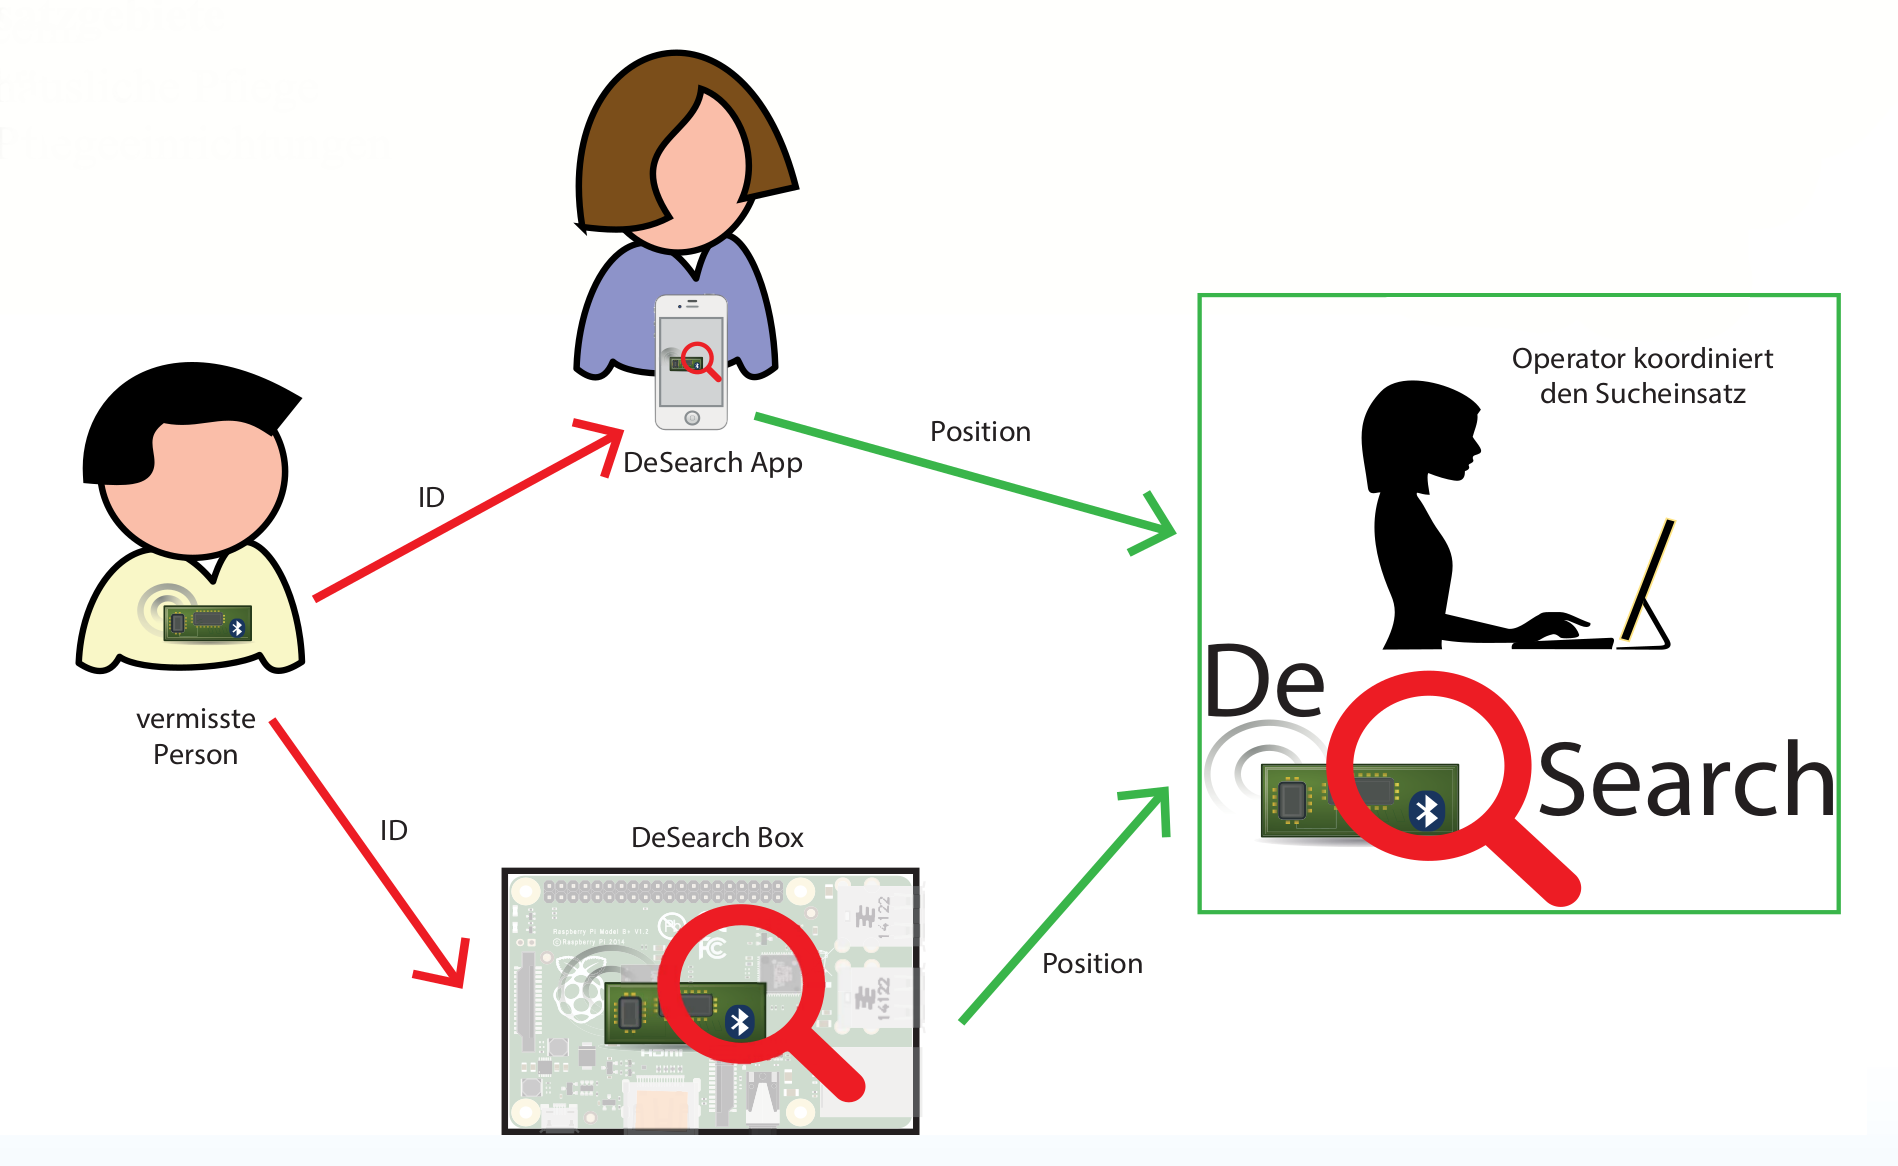
\includegraphics[width=\textwidth]{images/iCare-Systematik}
	\caption[Funktionsweise des DeSearch-Systems]{Schematische Darstellung der Funktionsweise des DeSearch-Systems, Quelle: http://www.bodenseehochschule.org/wp-content/uploads/2015/12/IBH\_ProjektPlakate\_A0\_iCare.pdf }
	\label{fig:desearch}
\end{figure} 
Im Rahmen dieser Projektarbeit soll ein lauffähiger Prototyp der Zentrale, der DeSearch-Boxen und der Web-Oberfläche erstellt werden, der dann in einer Testumgebung an der dualen Hochschule getestet werden soll.

	\section{Methodisches Vorgehen zur Problemlösung}

%%%%%%%%%%%%%%%%%%%%%%%%%%%%%%%%%%%%%%%%%%%%%%%%%%%%%%%%%%%%%%%%%%%%%%%%%%%%%%%%%%%%%%%%%%%%%%
\subsection{Aktueller Stand der Technologie}

\subsubsection{Bluetooth-Technologie}\label{sssec:BLE}
Bluetooth ist eine drahtlose Datenübertragunsgtechnologie, die basierend auf der Funktechnik Verbindungen zwischen Geräten über eine kurze Distanz ermöglicht. Im engen Nahbereich gilt Bluetooth als der Kommunikationsstandard \citep[Vgl.][S. 133]{mobil-sicher}. Mit dem Bluetooth Low Energy (BLE\nomenclature{BLE}{\textbf{B}luetooth \textbf{L}ow \textbf{E}nergy}) Standard, der 2009 verabscheidet wurde, konnte der Stromverbrauch für eine Bluetooth-Verbindung in den Endgeräten drastisch reduziert werden. Dies gelang unter anderem durch kürzere Verbindungsaufbauzeiten und Schlafphasen (Standby) zwischen den Sendezyklen. Eine vergleichende Untersuchung zum Energieverbrauch von Bluetooth und BLE veröffentlichten \cite{ble-energy}. 


\subsubsection{Raspberry Pi}\label{sssec:raspberry}
Für die Zentrale und die DeSearch-Boxen ist zunächst eine Hardware-Entscheidung notwendig. Benötigt werden Mikrocontroller oder Mikrocomputer mit folgenden Eigenschaften:
\begin{itemize}
	\item W-LAN Verbindung von der Box zur Zentrale möglich
	\item Bluetooth-fähige Box zur Markenerkennung
	\item Zentrale muss als Server fungieren und HTTP-Requests senden und verarbeiten können
	\item Datenbank-Installation zur Datenhaltung notwendig
\end{itemize}
Zudem sollen die Kosten pro Gerät so gering wie möglich gehalten werden. \\
Der Rasberry Pi ist ein Mikrocomputer mit einer Grundfläche, die etwas größer ist als eine Kreditkarte. In Abbildung \ref{fig:raspi} ist ein Raspberry Pi in der Draufsicht abgebildet.
\begin{figure}
	\centering
	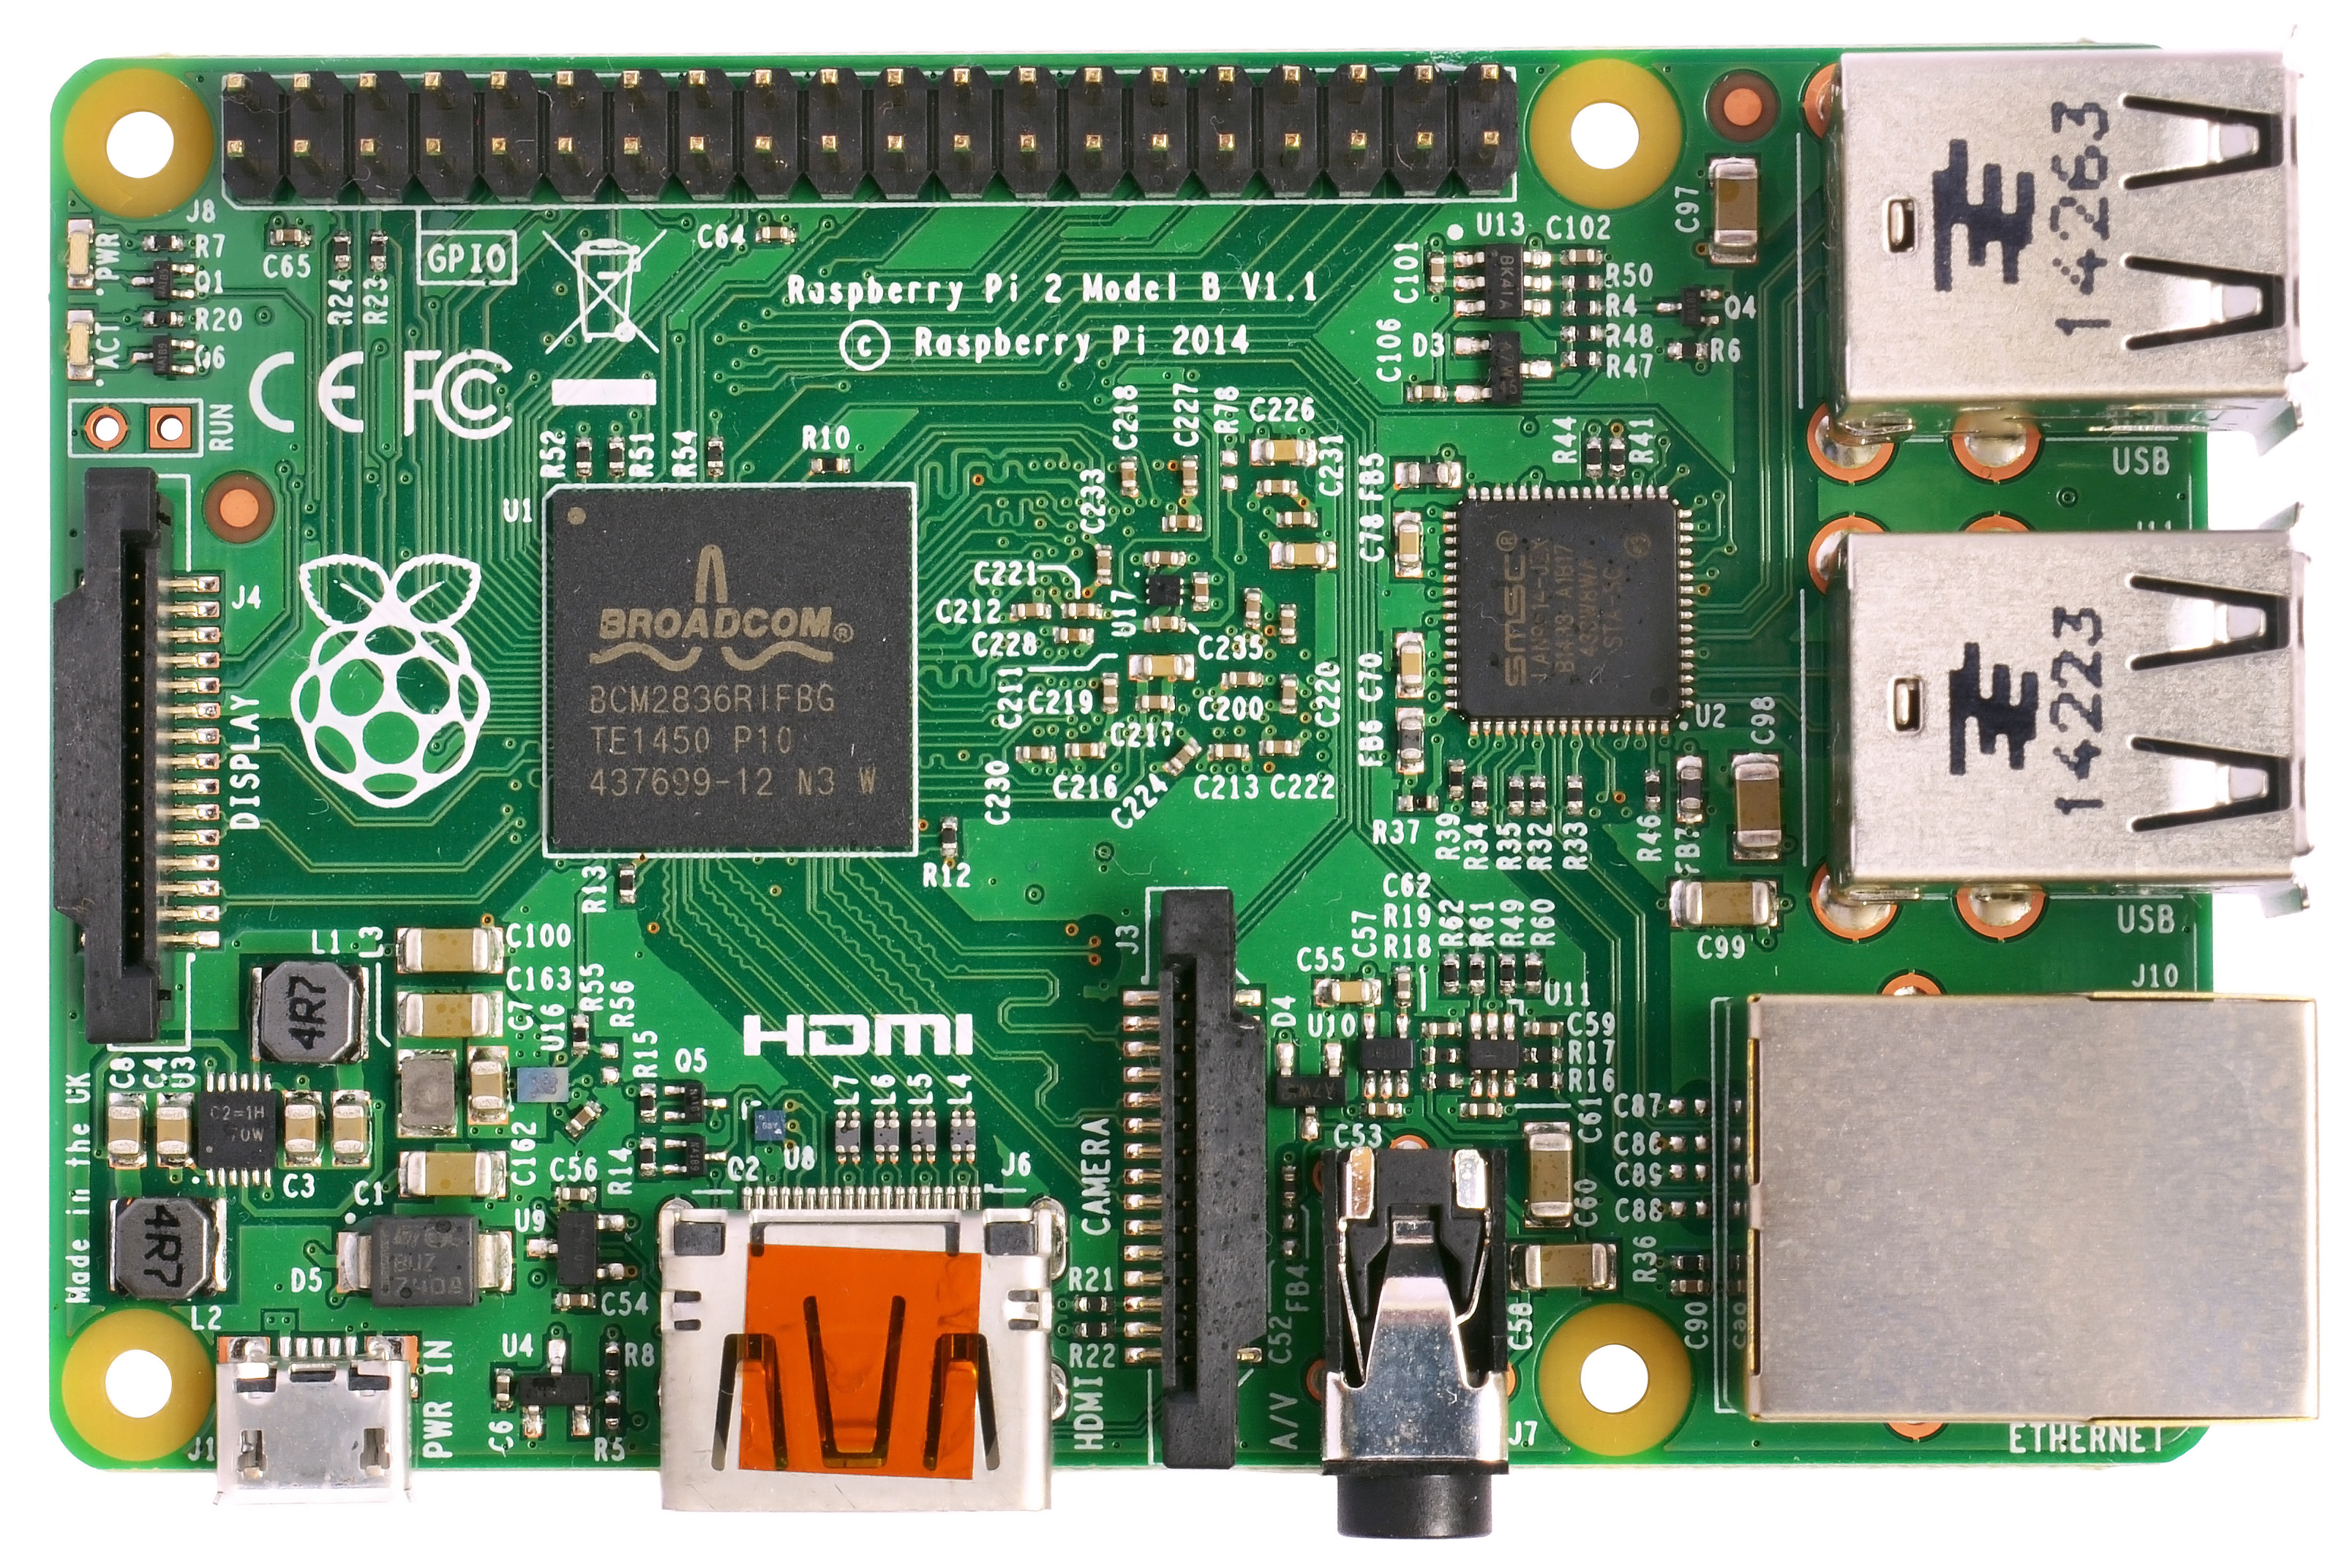
\includegraphics[width=1.0\linewidth]{images/Raspberrypi}
	\caption[Raspberry Pi in der Draufsicht]{Raspberry Pi Model 2, fungiert im DeSearch-Projekt als DeSearch-Box und als Zentrale, Quelle: https://en.wikipedia.org/wiki/Raspberry\_Pi}
	\label{fig:raspi}
\end{figure}
 Die Anschaffungskosten liegen ohne Zubehör bei etwa 42 €. Für diese geringen Anschaffungskosten erhält man einen vollwertigen, Linux-basierten Computer mit einer ARM-CPU, W-LAN und Bluetooth-Schnittstelle. Im Gegensatz zu Mikrocontrollern ist der Raspberry Pi leistungsfähiger und läuft stabiler \citep[Vgl.][S.35ff.]{raspi}. Auf einem Arduino-Mikrocontroller beispielweise kann nur C++-Code in einer Endlos-Schleife ausgeführt werden. Der Pi hingegen bietet die Möglichkeit, Bash-Skripte, Python-Code, Datenbank-Anfragen und Webserver gleichzeitig auszuführen. Die Entscheidung für den Raspberry Pi ist auch aufgrund der relativ niedrigen Anschaffungskosten für einen kompletten Rechner mit Betriebssystem gefallen. Für die Entwickler ist das Betriebssystem Linux zudem am einfachsten zu bedienen. Für das Projekt werden Pakete mit Raspberry Pi Model 2, SD-Karte, W-LAN und Bluetooth-Dongles, Netzteil und Gehäuse für ca. 75 € pro Paket angeschafft.
\subsubsection{Software-Rollout mit apt und dpgk}
Zum Installieren von Software wird unter Debian-basierten Systemen (dazu gehört neben Ubuntu und natürlich Debian selbst auch das Standardbetriebssystem des Raspberry Pi: Rasbian) das Programm \enquote{dpkg} verwendet.
Zur Installation eines Programms muss eine \enquote{.deb}-Datei vorliegen. Statt dem manuellen Download, der auch bei jedem Update erneut durchgeführt werden müsste, lässt sich zum Verteilen der \enquote{.deb}-Dateien \textbf{apt} verwenden.
Apt selbst nimmt keine Installation vor, es kümmert sich lediglich um die Beschaffung der aktuellsten \enquote{.deb}-Dateien und deren Abhängigkeiten (ebenfalls im \enquote{.deb} Format) und reicht diese zur Installation an dpkg weiter.
Neue Programme lassen sich mit \texttt{apt-get install <packetname>} installieren.
Dazu hält sich apt eine Liste mit allen verfügbaren Programmen in einem lokalen Cache vor. Um diese Liste zu aktualisieren, kann der Befehl \texttt{apt-get update} verwendet werden.
Dabei werden alle in der Datei \texttt{/etc/sources.list} bzw. dem Ordner \texttt{/etc/sources.list.d/} spezifizierten Quellen abgefragt.
Die Quellen werden dabei als URL angegeben und können unterschiedlichste Protokolle erfordern,
beispielsweise HTTP, HTTPS, FTP oder lokale Datenträger.
Zum Aktualisieren aller installierten Programme (nach dem Ausführen von \texttt{apt-get update}) wird der Befehl \texttt{apt-get upgrade} verwendet. Dabei wird die Softwareliste im Cache mit den installierten Programmen abgeglichen, ist eine aktuellere Version verfügbar wird deren \enquote{deb}-Paket heruntergeladen und mittels dpkg installiert.
\newline\textbf{apt}\newline
Zum Aktualisieren der Softwareliste lädt apt zunächst die Release Datei von der Quelle herunter. Diese ist mit gnupg signiert und enthält Informationen über die Paketquelle, wie z.B. die unterstützen CPU-Architekturen.
Außerdem sind Hash-Summen der Packages-Dateien enthalten, da diese nicht gnupg signiert sind.
Danach wird die Package-Datei heruntergeladen. Diese Datei ist spezifisch für eine Architektur und kann in einem Repository mehrfach vorkommen.
Sie enthält die Namen aller verfügbaren Pakete dieses Repositories sowie deren Abhängigkeiten, Beschreibung, Pfad und Hash-Werte der zugehörigen \enquote{.deb}-Datei sowie weitere Metadaten.
\newline\textbf{dpkg}\newline
dpkg installiert, konfiguriert und deinstalliert \enquote{deb}-Pakete.
Eine \enquote{.deb}-Datei enthält in einem Archiv alle Dateien, die das zu installierende Programm zur Ausführung benötigt.
Außerdem sind in einem weiteren Archiv verschiedene Kontrolldateien enthalten. Eine davon enthält Metadaten wie Namen des Pakets, Abhängigkeiten und der Beschreibung.
Daneben sind (optional) Skripte enthalten, die ausgeführt werden bevor oder nachdem das Paket installiert, deinstalliert oder aktualisiert wurde. 

\subsubsection{PostgreSQL}
PostgreSQL ist ein objektrelationales Datenbank-Management-System (DBMS), das aus dem Projekt POSTGRES der kalifornischen Universität Berkeley heraus entstanden ist. Der objektrelationale Ansatz bedeutet eine Erweiterung der relationalen DBMS um die Konzepte der Objektorientierung. Somit können in objektrelationalen DBMS beispielsweise komplexe Datenstrukturen mit Attributen definiert werden oder Vererbungen vorgenommen werden \citep[Vgl.][S. 135f.]{datenbanken}. In anderen DBMS muss hierfür \enquote{object relational mapping} (ORM) hinzugezogen werden, um Objektstrukturen auf relationale Tabellen abzubilden \citep[Vgl.][S. 426]{balzert}. Viele Konzepte, die in POSTGRES neu waren, wurden später in kommerzielle DBMS übernommen. PostgreSQL ist die Open-Source-Variante von POSTGRES und unterstützt einen großen Teil des SQL-Standards. Zudem bietet es Features wie komplexe Queries, Fremdschlüsselbeziehungen, Trigger, updatefähige Views und transaktionale Integrität. Außerdem kann der Benutzer PostgreSQL beliebig durch neue Datentypen, Funktionen, Operatoren oder Aggregationsfunktionen erweitern. Aufgrund der Open-Source-Lizenz kann PostgreSQL von jedem verwendet, verbessert oder verteilt werden
\nomenclature{DBMS}{\textbf{D}aten\textbf{b}ank \textbf{M}anagement \textbf{S}ystem}
\citep[Vgl.][preface, S. lxvi]{postgres}. Für das DeSearch-Projekt eignet sich PostgreSQL vor allem wegen seiner Open-Source-Lizenz, was die Kosten für das Projekt gering hält. Zudem ist die Möglichkeit, eigene Datentypen definieren zu können, von Vorteil. Da die Datenbank auf dem Zentral-Raspberry verwendet wird, der meist über SSH in der Konsole bedient wird, ist PostgreSQL einfach zu bedienen, da es über einen Konsolenclienten verfügt.

\subsubsection{Services unter Linux mit systemd}\label{sssec:systemd}
\textbf{systemd} ist ein Init-Tool unter Linux, das als neuere Alternative zu sysvinit und upstart gilt. Es ist für das Starten von Services und das Mounten von Hard Disks beim boot zuständig. Systemd verwaltet Hintergrunddienste (Daemons) und bietet ein Event-gesteuertes Starten von diesen, analog zum Runlevel-Prinzip von sysvinit. Dies bedeutet, dass bestimmte Gruppen von Services an bestimmten Punkten beim Boot gestartet werden, zum Beispiel sobald die GUI verfügbar ist oder sobald eine aktive Netzwerkverbindung besteht. In Tabelle \ref{tab:lvl} ist ein Vergleich zwischen den sysvinit-runlevels und den systemd-targets zu sehen. 
\begin{table}[h]
	\begin{tabular}{|p{2,5cm}|p{3,5cm} |p{8,5cm} | }
		\hline
		\textbf{sysvinit Runlevel} & \textbf{systemd-target} & \textbf{Bedeutung}\\ \hline
		0 & poweroff.target & System-Shutdown	\\ \hline
		1, single & rescue.target & Single-User-Modus \\ \hline
		2,4 & multi-user.target & Benutzerdefinierte runlevels, per default identisch mit runlevel 3 \\ \hline
		3 & multi-user.target & Multi-User-Umgebung, ohne graphische Benutzer\-oberfläche (Login über Konsole möglich)\\ \hline
		5 & graphical.target & Multi-User-Umgebung, graphische Benutzer\-oberfläche \\ \hline
		6 & reboot.target & System-Reboot \\ \hline
		emergency & emergency.target & Emergency Shell\\ \hline
		
	\end{tabular}
	\caption[Übersicht über die targets von systemd]{Übersicht über die targets von systemd, in Anlehnung an \cite{fedora}}
	\label{tab:lvl}
\end{table}
Mithilfe dieser targets können beispielsweise voneinander abhängige Hintergrundservices nacheinander gestartet werden. Neben den runlevels entsprechenden targets gibt es noch einige weitere, wie zum Beispiel das \textbf{network-online.target}.
Auch der Raspberry Pi mit Raspbian verwendet systemd. Für die DeSearch-Boxen eignet es sich, um den Scan-Vorgang als Hintergrundprozess zu verwalten und so sicherzugehen, dass dieser stabil läuft und nach eventuellem Reboot oder Verbindungsabbruch selbständig wieder startet.\newline
Über die Konsole kann \textbf{systemctl} aufgerufen werden. Dies ist die Überwachungs- und Steuereinheit von systemd. Mit \texttt{systemctl start xyz.service} kann ein Service gestartet werden. Respektive kann mit  \texttt{systemctl restart xyz.service} und \texttt{systemctl stop xyz.service} der Service neugestartet oder angehalten werden. Mit  \texttt{systemctl status xyz.service} wird eine Ausgabe erzeugt, die über den Status des Service informiert und eventuelle Ausgaben des Service anzeigt. Diese Kommandos und alle weiteren Optionen von systemctl befinden sich im Manual \citep[][]{systemctl-man}.

\subsection{Umsetzung der Anforderungen}
Die Umsetzung der prototypischen Implementierung teilt sich in viele Unterthemen auf. Zur Übersicht ist in Abbildung \ref{fig:architektur} die Architektur des DeSearch-Systems mit den einzelnen Komponenten abgebildet.
\begin{figure}[bth]
	\centering
	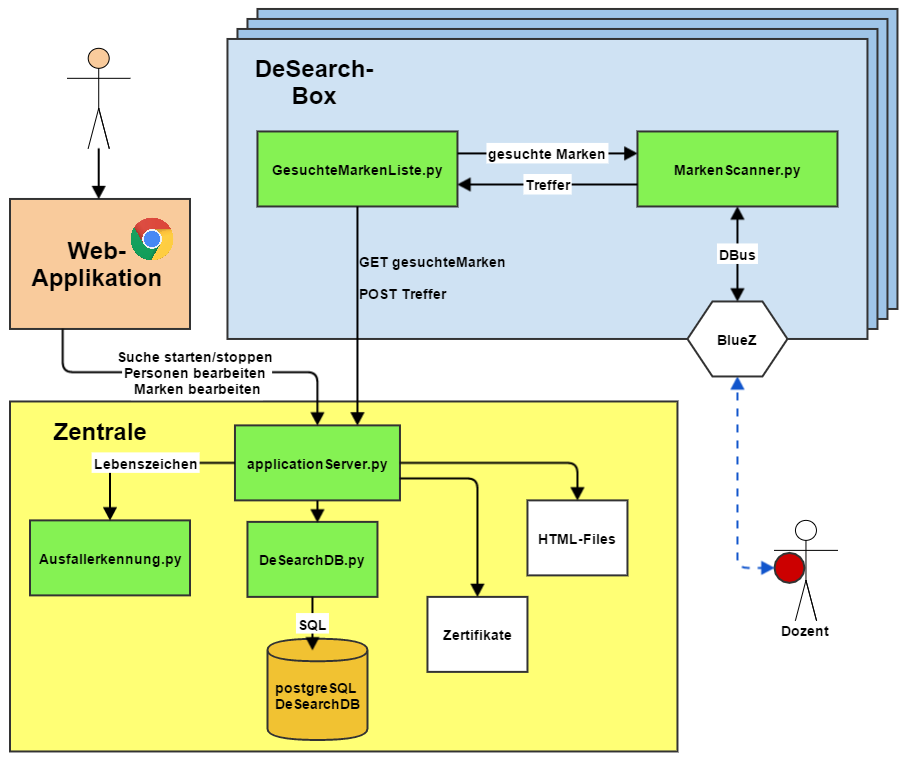
\includegraphics[width=1.0\linewidth]{images/schichten.png}
	\caption[Architektur des DeSearch-Systems]{Architektur des DeSearch-Systems, Quelle: eigene Darstellung}
	\label{fig:architektur}
\end{figure}
In den grünen Blöcken sind die python-Module dargestellt, aus denen die Software aufgebaut ist. \textbf{Die Zentrale} dient als HTTP-Server sowohl für die Web-Applikation als auch für die Kommunikation mit den DeSearch-Boxen. Die Kommunikation erfolgt abgesichert über HTTPS (siehe auch Kapitel \ref{cap:authentifizierung}). In \enquote{applicationServer.py} werden alle Anfragen verarbeitet. Dieses Modul wird als Service automatisch auf der Zentrale gestartet und am Laufen gehalten (siehe auch Kapitel \ref{sssec:services}). Die Kommunikation zur Datenbank wird an \enquote{DeSearchDB.py} weitergegeben. Dieses Modul stellt einen Adapter zu der installierten PostgreSQL-Datenbank dar, der die Anfragen in SQL-Anfragen umwandelt und in die Datenbank hineingibt. Nähere Details zum Datenbankschema finden sich in Kapitel \ref{sssec:db}. Das Modul \enquote{Ausfallerkennung.py} ist dafür zuständig, die Lebenszeichen der DeSearch-Boxen zu verarbeiten. Dies dient der Überwachung des Systemstatus.\\
In den \textbf{DeSearch-Boxen} laufen zwei Python-Skripte in parallelen Threads. \enquote{GesuchteMarkenListe.py} fragt in regelmäßigen Abständen bei der Zentrale an, welche Marken momentan gesucht werden. \enquote{MarkenScanner.py} verarbeitet die Ergebnisse des Bluetooth-Scan, der ständig läuft. Hierfür wird der Bluetooth-Stack \enquote{BlueZ} verwendet (siehe Kapitel \ref{sssec:bluez}). Anschließend werden die Ergebnisse mit den gesuchten Marken verglichen.  Ein Treffer wird an \enquote{GesuchteMarkenListe.py} zurückgegeben. Dieses Modul meldet den Treffer dann mittels POST an die Zentrale weiter. Die Web-Applikation wird auch vom applicationServer aus gespeist, denn die HTML-Dokumente liegen auf der Zentrale. Über die Web-Anwendung können alle administrativen Tätigkeiten wie das Starten und Stoppen einer Suche, das Anlegen und Bearbeiten von Personen, das Hinzufügen von Marken und die Systemüberwachung ausgeführt werden (siehe Kapitel \ref{sssec:ui}). 


\subsubsection{Authentifizierung} \label{cap:authentifizierung}
Im System gibt es 4 verschiedene Authentifizierungen (vgl. Tabelle \ref{tab:authentifizierungen}).\newline
Die \textbf{Zentrale} authentifiziert sich bei den Nutzern und Boxen (Authentisierende) mittels SSL-Zertifikat, wie jeder Webserver der im Internet über HTTPS zur Verfügung steht. Aktuell handelt es sich dabei um ein selbst signiertes Zertifikat, das auf den Boxen und den Endgeräten der Nutzer manuell eingespielt werden muss. Ist die DeSearch-Zentrale zukünftig über eine globale Domain erreichbar, kann auch ein Zertifikat bei einer Root CA beantragt werden, welcher die Browserhersteller vertrauen. \newline
Die \textbf{Boxen} authentifizieren sich gegenüber der Zentrale ebenfalls mittels eines SSL-Zertifikates.
Dieses muss beim Installieren der Box zwischen Zentrale und Box ausgetauscht werden. \\Dazu wird auf der Box das Python-Script \texttt{/opt/desearch-client/keyExchange.py} und der Zentrale die Serverversion des Scripts \texttt{/opt/desearch-server/keyExchange.py} mit root-Berechtigung gestartet. Daraufhin tauschen Server und Klient ihre Zertifikate aus und zeigen deren Hashwerte an. Die Übereinstimmung ist dann zu prüfen um MITM-Attacken auszuschließen. Nach Bestätigen der Gleichheit werden die Zertifikate abgespeichert. \newline
\textbf{Nutzer} authentifizieren sich bei der Zentrale mit einer Nutzername / Passwort Kombination. Danach erstellt die Zentrale ein Token, das für alle weiteren Anfragen verwendet wird. Das Token wird selbstverständlich transparent für den Nutzer vom JavaScript-Code des Use-Interfaces entgegengenommen, verwaltet und mitgesendet.

\begin{table}[h]
	\begin{tabular}{ | l | l | l | l |}
		\hline
		\textbf{Zeile} & \textbf{Authentifizierender} & \textbf{Authentisierender} &  \textbf{Methode} \\ \hline
		1 & Zentrale & Box      & SSL Klient Zertifikat \\ \hline
		2 & Zentrale & Nutzer   & Nutzername, Passwort, Token \\ \hline
		3 & Box      & Zentrale & SSL Server Zertifikat \\ \hline
		4 & Nutzer   & Zentrale & SSL Server Zertifikat \\ \hline
		
	\end{tabular}
	\caption{Authentifizierungen im System}
	\label{tab:authentifizierungen}
\end{table}

\subsubsection{Erkennen der Marken über Bluetooth}\label{sssec:bluez}
Durch die eingschränkte Sendereichweite von Bluetooth soll die Ortung im DeSearch-Projekt gelingen. Die dementen Patienten tragen kleine BLE-Sendemarken am Körper, die von den fest installierten DeSearch-Boxen erkannt werden, sobald sich der Patient in der Nähe aufhält. So kann auf den ungefähren Aufenthaltsort der Person geschlossen werden, sobald eine der Boxen einen Treffer an die Zentrale meldet. \newline
Als Ergebnis eines studentischen Workshops auf der Hütte in Balderschwang gibt es eine Python-Klasse, die einen BLE-Scan starten kann und basierend auf einer Liste von MAC-Adressen eine Callback-Funktion aufruft, wann immer eine der MAC-Adressen in der Liste gesichtet wird.
Diese Klasse verwendet die Bibliothek "bleep", die sich allerdings im Laufe der Projektarbeit als nicht geeignet herausstellte, da sie folgende Probleme aufweist:
\begin{itemize}
	\item Wird sie nicht mit root-Rechten ausgeführt, kommt es zum Absturz.
	\item Die Installation ist für eine großflächige Verteilung zu aufwändig und erfordert unter anderem die Installation einer modifizierten Version von "pygattlib" \citep[Vgl.][]{bleep-installation}.
	\item Es handelt sich dabei um ein Ein-Mann-Projekt, dessen Entwickler die Bibliothek aus einem privaten Bedürfnis heraus geschaffen hat. Damit ist die Softwarequalität und Wartung abhängig von einer einzelnen Person.
\end{itemize}
Zur Bluetooth-Kommunikation unter Linux kann der im Linux Kernel enthaltene Bluetooth Stack "BlueZ" verwendet werden. Dieser enthält auch Treiber für die meisten Bluetooth Chipsets.
Auch die bleep-Bibliothek verwendet BlueZ. Im Rahmen der Projektarbeit erfolgt eine Reimplementierung der Scanner-Klasse in Python, die ohne die Verwendung von bleep auskommt.
In der Reimplementierung wurden dabei die Schnittstellen der Klasse erhalten, die Kommunikation mit BlueZ findet nun über den DBus statt. Dies erfordert keine root-Rechte und ist neben den Kommandozeilen-Tools der einzig im offiziellen Git-Repository von BlueZ dokumentierte Weg zum Ansprechen der Schnittstellen \citep[Vgl.][]{bluez-git}. Außerdem werden damit nur noch die DBus-Bibliothek von Python und BlueZ auf den DeSearch-Boxen benötigt, diese sind in den offiziellen Paketquellen enthalten und damit einfach zu verteilen und zu aktualisieren.

\subsubsection{Robustheit des Systems durch Services}\label{sssec:services}
Um eine gewisse Robustheit des Systems zu gewährleisten, muss sichergestellt werden, dass die Python-Skripte zum Scan auf den DeSearch-Boxen sowie die Python-Skripte des Web-Servers auf der Zentrale immer laufen. Dies wird durch Hintergrundservices realisiert. Anforderung an die Services ist es, dass sie sich nach einem Reboot selbständig starten und nach einem unerwarteten Fehler oder Ausführungs-Stop selbständig re-spawnen(d.h. sich selbst neu-starten). Realisiert wurde dies durch systemd-Services, welche in Kapitel \ref{sssec:systemd} bereits erläutert wurden. Die Konfiguration innerhalb des Service ist für Zentrale und DeSearchBox gleich, da die Anforderungen auch gleich sind. Um einen Hintergrundservice anzulegen, muss zunächst das \texttt{.service}-File unter dem Pfad \texttt{/lib/systemd/system/} angelegt werden. In diesem Verzeichnis werden alle Services von systemd nachgeschlagen. Beispielhaft ist in Abbildung \ref{fig:service} das Service-File der DeSearch-Zentrale zu sehen.
\begin{figure}[bth]
	\centering
	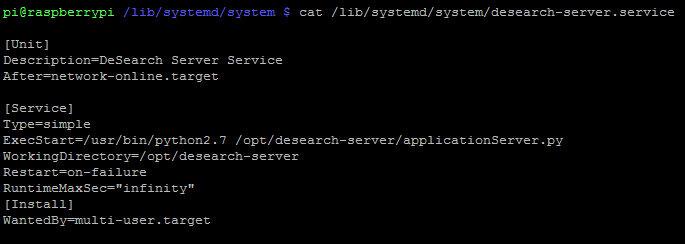
\includegraphics[width=1.0\linewidth]{images/service-systemd}
	\caption[Service-File auf dem Zentral-Pi]{Service-File auf dem Raspberry Pi, der als Zentrale fungiert.}
	\label{fig:service}
\end{figure}
Zunächst werden unter \texttt{[Unit]} Informationen zu dieser Service-Unit aufgeführt. Dies ist die Beschreibung des Service (unter Description) und die Information, wann der Service beim Boot gestartet werden soll. Hier stehen unter Anderem die Optionen \enquote{Before} und \enquote{After} zur Verfügung. Im \texttt{desearch-server.service} wird durch \enquote{After=network-online.target} ausgedrückt, dass der Service erst gestartet werden darf, wenn eine aktive Netzwerkverbindung besteht (siehe auch Kapitel \ref{sssec:systemd}). Ansonsten wird der Start des Service verzögert, bis die angegebene Bedingung erfüllt ist.
In der darauf folgenden \texttt{[Service]}-Sektion wird angegeben, was der Hintergrundservice tun soll. Die Angabe des \enquote{simple}-Type bewirkt, dass der Prozess, den der Service startet, auch dessen Haupt-Prozess ist. Anders verhält es sich, wenn hier \enquote{forking} gewählt wird: Dann verhält sich der Prozess wie ein traditioneller UNIX-Daemon und startet als Kindprozess des Service. \\
Nach der Angabe des Typs wird unter \enquote{ExecStart} angegeben, was der Service ausführen soll. Hier wird zunächst der Pfad der Python-Installation angegeben und anschließend der Pfad des deSearch-Server-Skripts, das von Python ausgeführt werden soll. Zusätzlich wird noch ein Working-Directory angegeben, da Python sonst von dem Service im Root-Verzeichnis gestartet wird und dann die restlichen benötigten Python-Skripte nicht gefunden werden. \\
Der nächste Parameter, \enquote{Restart}, bestimmt wann der Service neu gestartet werden soll. Hier gibt es verschiedene Optionen, die in der man-Page von systemd nachgeschlagen werden können (vgl. \cite{systemd-service}). Für lang laufende Hintergrundprozesse empfiehlt die man-Page die Wahl von \enquote{Restart=on-failure}. Der Service wird bei unsauberen Exit-Codes (ungleich 0), wenn er von einem Signal beendet wird (z.B. Core Dump), bei einem Timeout oder (falls konfiguriert) bei fehlendem Watchdog-Signal neu gestartet. Die maximale Laufzeit des Service wird zudem im nächsten Argument \enquote{RuntimeMaxSec} auf unendlich gesetzt.\\
Im \texttt{[Install]}-Abschnitt wird abschließend festgelegt, welche Abhängigkeiten ein Service hat. Die Angabe \enquote{multi-user.target} stellt eine Abhängigkeit her, die bewirkt, dass der Service dann gestartet wird, wenn auch die Multi-User-Umgebung gestartet wird. \\
Nach dem Anlegen des Service-Files wird \texttt{systemctl daemon-relaod} einmalig ausgeführt, um anschließend mit \texttt{systemctl enable desearch-server.service} den Service zu aktivieren. Nun kann entweder durch einen reboot der Service automatisch gestartet werden (wie konfiguriert) oder mittels \texttt{systemctl start desearch-server.service} auch manuell. Abbildung \ref{fig:systemctl-status} zeigt die Statusausgabe von Systemctl nach erfolgreichem Start des Service.
\begin{figure}[bth]
	\centering
	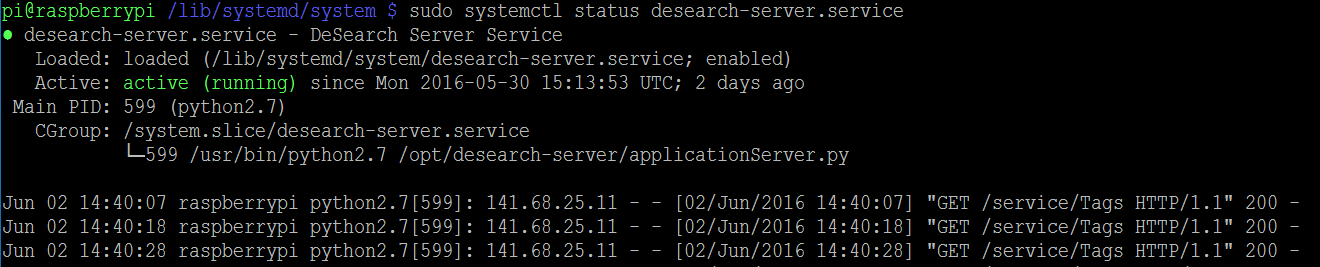
\includegraphics[width=1.0\linewidth]{images/service-status}
	\caption[Status-Ausgabe von Systemctl]{Status-Ausgabe von Systemctl für den deSearch-Zentral-Service.}
	\label{fig:systemctl-status}
\end{figure}

\subsubsection{Datenbankschema}\label{sssec:db}
In Abbildung \ref{img:db-schema} ist das Datenbankschema zu sehen, mit dem die Zentrale arbeitet. 
\begin{figure}
	\centering
	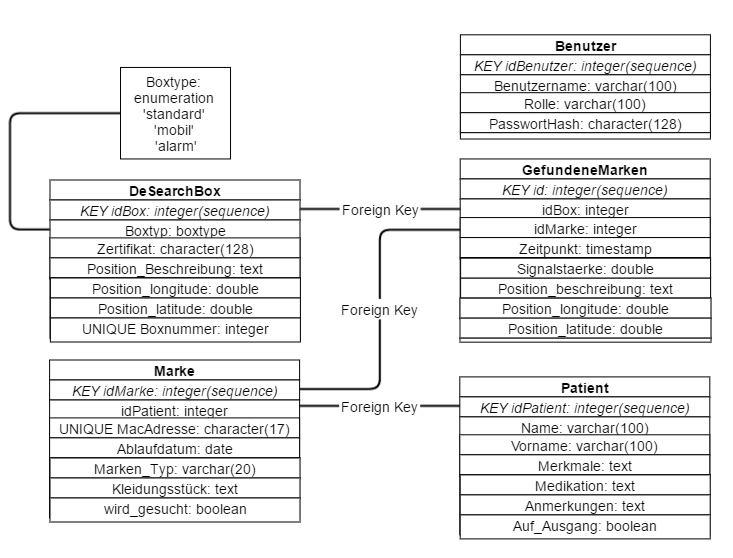
\includegraphics[width=1.0\linewidth]{images/db-schema}
	\caption[Datenbankschema der Zentrale]{Datenbankschema der Zentrale, Quelle: eigene Darstellung}
	\label{img:db-schema}
\end{figure}
\begin{itemize}
\item Für den Zugang zur Web-Oberfläche werden \textbf{Benutzer} mit ihren Rollen in der Datenbank angelegt. Das Passwort wird dabei als Hash mit 128 Zeichen in der Datenbank gespeichert. 
\item Jede \textbf{DeSearch-Box} wird in der Datenbank mit ihrer Position und Boxnummer angelegt. Für die Zukunft wurde bereits das Feld \enquote{Boxtyp} erstellt, da im weiteren Verlauf ortsfeste, mobile und Alarm-Boxen unterschieden werden sollen. Bei mobilen Boxen (z.B. im Auto, in Linienbussen) wird anstatt einer festen Positionsbeschreibung die genaue Geo-Location mit Longitude und Latitude ermittelt. Alarm-Boxen können beispielsweise am Hof-Ausgang oder an der Bushaltestelle installiert werden und standardmäßig immer Alarm auslösen, wenn dort eine Marke gefunden wird.
\item Die \textbf{Marken} werden in der Datenbank mit einer eindeutigen MAC-Adresse abgelegt, die beim Abgleich mit den Scan-Ergebnissen verwendet wird. Außerdem wird die ID des zugehörigen Patienten vermerkt und ein Hinweis auf das jeweilige Kleidungsstück, in das die Marke eingenäht ist. Zusätzlich wird ein Ablaufdatum in die Datenbank eingetragen, das den ungefähren Zeitpunkt des nächsten Batteriewechsels festhält. Somit kann eine Warnmeldung angezeigt werden, wenn der Batteriewechsel fällig ist. Ein wichtiges Feld ist der boolean \enquote{wird\_gesucht}. Wird auf der Web-Oberfläche eine Suche gestartet, so werden alle zu dieser Person gehörigen Marken auf wird\_gesucht gesetzt. Nur dann werden Treffer zu dieser Person von den Boxen an die Zentrale gemeldet. Finden die Suchenden beispielsweise nur ein Kleidungsstück der vermissten Person, können einzelne Marken gezielt von der Suche ausgeschlossen werden. 
\item Ein \textbf{Patient} liegt in der Datenbank mit Name, Vorname und weiteren für die Suche wichtigen Informationen vor. Beispielsweise kann unter \enquote{Merkmale} die Beschreibung einer Person vermerkt werden, unter \enquote{Medikation} und \enquote{Anmerkungen} können wichtige Hinweise im Fall eines Fundes oder einer längeren Abwesenheit der Person gespeichert werden. Gerade bei Diabetikern oder Patienten, die regelmäßig Medikamente nehmen müssen, ist diese Information besonders wichtig. Das Flag \enquote{Auf\_Ausgang} kann gesetzt werden, falls ein Angehöriger mit der Person das Pflegeheim verlässt, beispielsweise für einen Spaziergang. Somit wird ein Fehlalarm verhindert.
\item Die Tabelle \textbf{GefundeneMarken} kann eine Suchaktion protokollieren. Jeder Treffer, den eine Box registriert und an die Zentrale sendet, wird hier dokumentiert. Ein Treffer wird mit der zugehörigen BoxID, der MarkenID, dem Zeitpunkt und der Position in die Datenbank gelegt. Somit können auf der Web-Oberfläche alle Treffer in einer Zeitreihe angezeigt werden. Aus Datenschutzgründen werden die Einträge in dieser Tabelle nach jeder abgeschlossenen Suchaktion gelöscht.

\end{itemize}
\subsubsection{Benutzeroberfläche}\label{sssec:ui}
Die Benutzeroberfläche wurde unter Verwendung des Frameworks \textbf{Polymer} erstellt. Dieses zeichnet sich vor allem dadurch aus, dass es die Erstellung eines \enquote{responsive UI}, also einer Nutzerschnittstelle, die sich auf Smartphones, Tabletcomputern, Laptops sowie Desktop PC gleichermaßen bedienen lässt, unterstützt.\newline
Nachdem sich der Nutzer eingeloggt hat (vgl. Abbildung \ref{img:ui/login}) sieht er eine Liste aller Patienten im System. Patienten, nach denen aktuell gefahndet wird, werden dabei mit einem roten Icon hervorgehoben (vgl. Abbildung \ref{img:ui/personenliste}). Eine Liste, die nur die gesuchten Patienten enthält, lässt sich über das Menü aufrufen (vgl. Abbildung \ref{img:ui/menu}). \newline
Wählt der Nutzer in einer der Listen einen Patienten aus, so bekommt er weitere Details und verfügbare Aktionen angezeigt. Bei den Details handelt es sich um zuvor hinterlegten Informationen, wie das Aussehen und die Anmerkungen, sowie die Sichtungen im Falle einer aktiven Fahndung. Verfügbare Aktionen sind das Starten bzw. Stoppen einer Fahndung, das Löschen und Bearbeiten des Patienten und die Verwaltung der Marken (vgl. Abbildung \ref{img:ui/persondetails}). \newline
Startet der Nutzer die Markenverwaltung, so bekommt er zunächst die für den Patienten hinterlegten Marken aufgelistet und kann diese entfernen oder als gefunden markieren (vgl. Abbildung \ref{img:ui/markenverwalten}). Außerdem hat er die Möglichkeit dem Patienten eine neue Marke zuzuordnen (vgl. Abbildung \ref{img:ui/markehinzufuegen}). \newline
Neue Patienten werden über einen Button in der Liste hinzugefügt. Dieser öffnet ein Dialogfenster, in dem Details zum Patienten hinterlegt werden können (vgl. Abbildung \ref{img:ui/personhinzufuegen}).\newline
Der dritte Menüpunkt, der "System Monitor", bietet Informationen zum Status des Systems. Dort kann auf die Logdaten des Servers zugegriffen werden und die Zeit seit dem letzten Lebenszeichen der einzelnen DeSearch-Boxen steht zur Verfügung. In Abbildung \ref{img:ui/systemMonitor} ist der Systemmonitor bei einem simulierten Ausfall des \enquote{pi9} zu sehen. Im unteren Teil des Screenshots ist der Log des Servers zu sehen, dieser enthält in diesem Fall nur geloggte HTTP-Anfragen, dort wären aber auch unbehandelte Exceptions zu sehen.

\begin{figure}
	\centering
	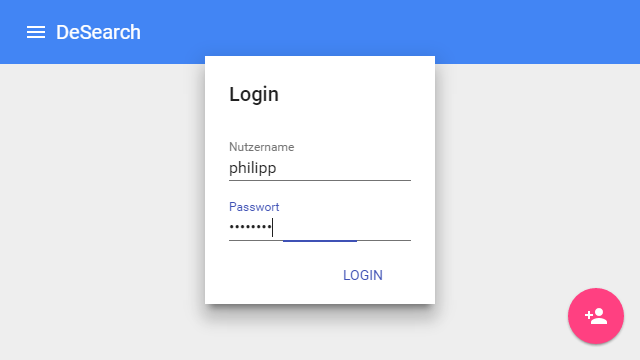
\includegraphics[width=1.0\linewidth]{images/ui/login}
	\caption[Benutzeroberfläche: Login]{Login}
	\label{img:ui/login}
\end{figure}

\begin{figure}
	\centering
	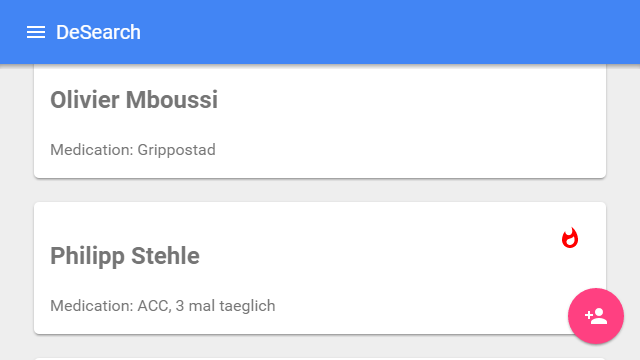
\includegraphics[width=1.0\linewidth]{images/ui/personenliste}
	\caption[Benutzeroberfläche: Liste aller Patienten]{Liste aller Patienten}
	\label{img:ui/personenliste}
\end{figure}

\begin{figure}
	\centering
	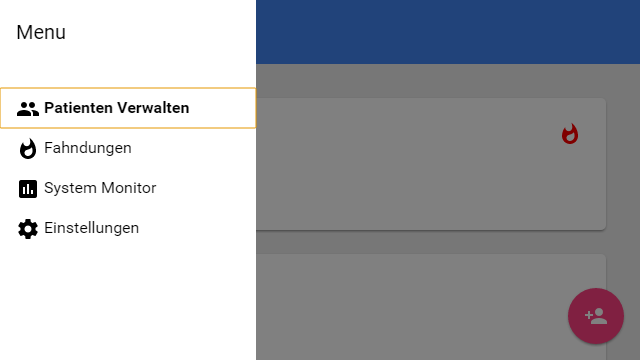
\includegraphics[width=1.0\linewidth]{images/ui/menu}
	\caption[Benutzeroberfläche: Menü]{Menü}
	\label{img:ui/menu}
\end{figure}

\begin{figure}
	\centering
	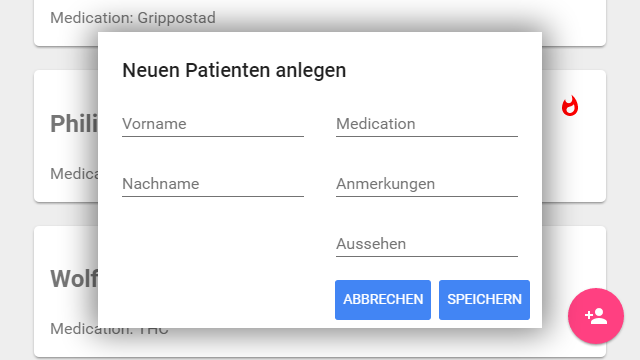
\includegraphics[width=1.0\linewidth]{images/ui/personhinzufuegen}
	\caption[Benutzeroberfläche: Patient anlegen]{Patient anlegen}
	\label{img:ui/personhinzufuegen}
\end{figure}

\begin{figure}
	\centering
	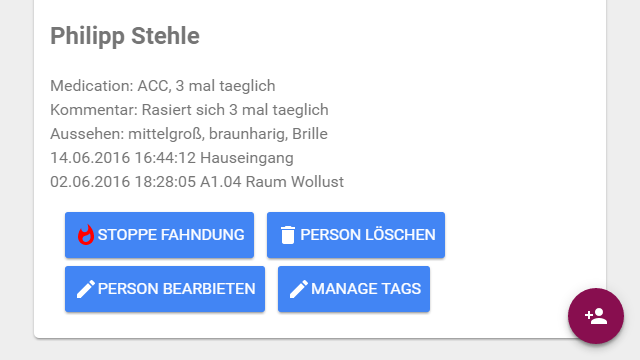
\includegraphics[width=1.0\linewidth]{images/ui/persondetails}
	\caption[Benutzeroberfläche: Details zu einem Patienten anzeigen]{Details zu einem Patienten anzeigen}
	\label{img:ui/persondetails}
\end{figure}

\begin{figure}
	\centering
	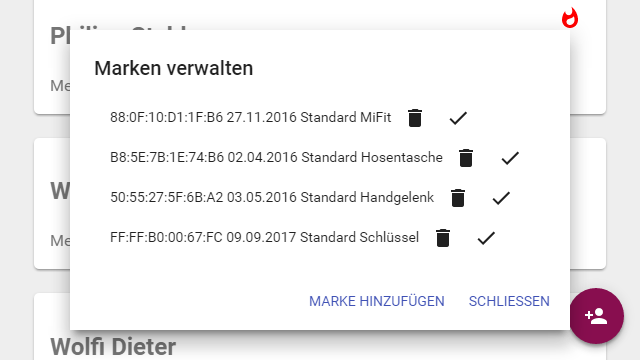
\includegraphics[width=1.0\linewidth]{images/ui/markenverwalten}
	\caption[Benutzeroberfläche: Marken eines Patienten verwalten]{Marken eines Patienten verwalten}
	\label{img:ui/markenverwalten}
\end{figure}

\begin{figure}
	\centering
	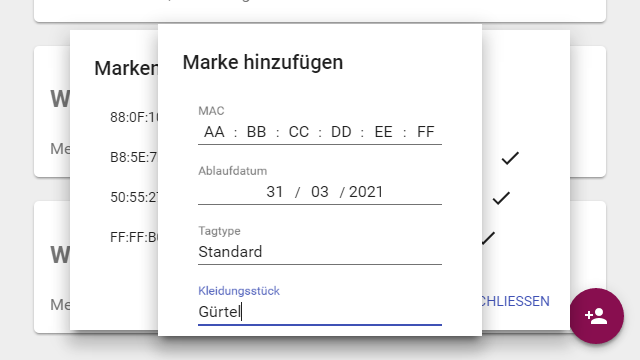
\includegraphics[width=1.0\linewidth]{images/ui/markehinzufuegen}
	\caption[Benutzeroberfläche: Neue Marken einem Patienten zuordnen]{Neue Marken einem Patienten zuordnen}
	\label{img:ui/markehinzufuegen}
\end{figure}


\begin{figure}
	\centering
	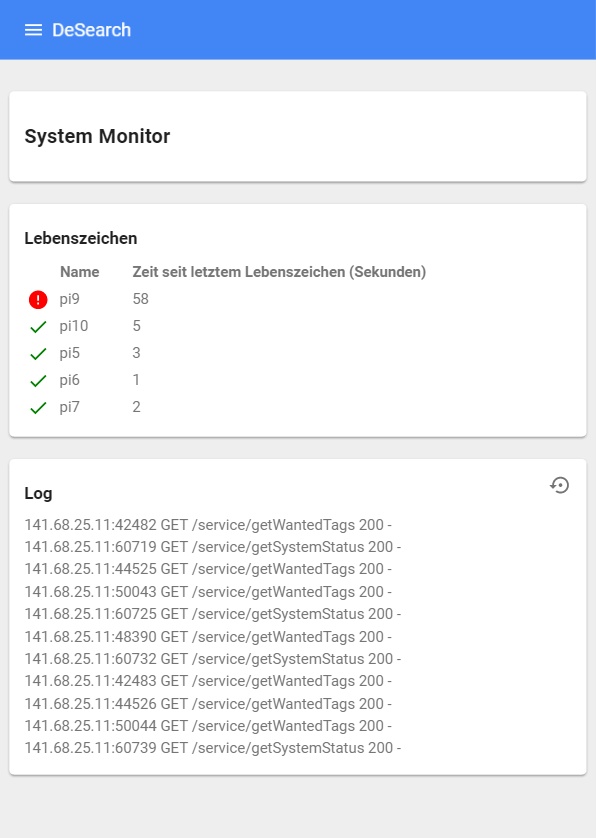
\includegraphics[width=1.0\linewidth]{images/ui/systemMonitor}
	\caption[Benutzeroberfläche: System Monitor]{System Monitor - Beispiel für Ausfall von \enquote{pi9}}
	\label{img:ui/systemMonitor}
\end{figure}


\subsubsection{Administrative Benutzeroberfläche}
In der aktuellen Umsetzung gibt es noch keine Administrative Benutzeroberfläche. Zum Hinzufügen und Löschen von Nutzern steht allerdings ein Skript zur Verfügung, das unter  \texttt{/opt/desearch-server/userManagement.py} ausgeführt werden kann (vgl. Abbildung \ref{img:userManagement}).
Das Einlernen einer neuen Box wird über das in Kapitel \ref{cap:authentifizierung} erwähnte Verfahren durchgeführt.

\begin{figure}
	\centering
	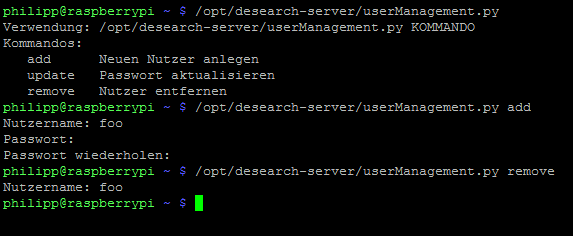
\includegraphics[width=1.0\linewidth]{images/userManagement}
	\caption[Nutzermanagement auf der Zentrale]{Nutzermanagement auf der Zentrale unter der Verwendung des Scripts "/opt/desearch-server/userManagement.py". Das Passwort wird dabei während der Eingabe nicht angezeigt.}
	\label{img:userManagement}
\end{figure}


\subsubsection{Infrastruktur und Netzwerk-Einschränkungen in der Testumgebung}\label{sssec:tunnel}
Die Raspberry Pi's werden in der DHBW Ravensburg am Campus Friedrichshafen zum Testbetrieb installiert. Dabei fungiert ein Pi als Zentrale und die anderen als DeSearch-Boxen, die die Funde an die Zentrale melden. In Tabelle \ref{tab:pis} ist eine Übersicht über alle installierten Raspberry Pi's aufgelistet.
Dazu wurde vom Netzwerkadministrator der DHBW die Erlaubnis eingeräumt, die vorhandene Infrastruktur zu verwenden. Daran geknüpft sind allerdings folgende Bedingungen bzw. Einschränkungen:
\begin{itemize}
	\item Zugriffe aus dem Internet sind nicht erlaubt.
	\item Alle Pi's außer der Zentrale (Slaves) verbinden sich über WLAN unter Verwendung speziell eingerichteter Zugangsdaten mit dem Netzwerk.
	\item Die Zentrale bekommt einen LAN Anschluss und eine feste IP Adresse plus DNS Eintrag zugewiesen.
	\item Ein Verbindungsaufbau zu den Slaves ist nicht möglich - jegliche Kommunikation muss von ihnen initiiert werden.
\end{itemize}
Die letzte Bedingung stellt eine Herausforderung dar, da damit auch kein SSH-Zugriff auf die DeSearch-Boxen möglich ist, der benötigt wird um die DeSearch Anwendung zu aktualisieren, starten oder überwachen.
Dieses Problem kann gelöst werden, da mit der Zentrale ein Gerät im Netzwerk ist, das für alle anderen Pi's und auch die zur Entwicklung und Wartung verwendeten Laptops erreichbar ist. Somit kann über die Zentrale ein Tunnel aufgebaut werden.
Zum Aufbauen des Tunnels bietet sich die Verwendung der SSH Portforwarding Funktion an, da alle beteiligten Geräte bereits für die Verwendung von SSH eingerichtet sind. Eine schematische Darstellung der Vorgehensweise ist in Abbildung \ref{fig:tunnel} zu sehen.
Zum Verbindungsaufbau wurde ein technischer Benutzer mit dem Namen "tunnel" auf der Zentrale angelegt, der sich über SSH und Zertifikat Authentifizierung einloggen kann.
Jeder Slave erhält einen RSA Schlüssel, den er zum Login verwenden kann, und über einen Eintrag in der Crontabelle wird sichergestellt, dass der Tunnel immer offen gehalten wird.
Der Ausgangsport des Tunnels ist dabei für jede DeSearch-Box eindeutig. Soll nun eine Verbindung zu einer Box hergestellt werden, so muss erst eine SSH Verbindung zur Zentrale aufgebaut werden und dort eine SSH Verbindung zum Eingang des Tunnels (localhost plus Tunnel Ausgangport) hergestellt werden.
\begin{table}[h]
	\begin{tabular}{ | p{2,5cm} | p{2,5cm} | p{4cm} | p{6cm} |}
		\hline
		\textbf{Pi-Nummer} & \textbf{Funktion} & \textbf{Installationsort} &  \textbf{Erreichbarkeit} \\ \hline
		3 & Zentrale & Büro Herr Judt & statische IP 141.68.30.39 oder \mbox{Judt-Master.it.ba-ravensburg.de} \\ \hline
		5 & DeSearch-Box & Haupteingang oberhalb der Treppe & Tunnel über Zentrale, Port 19005 \\ \hline
		6 & DeSearch-Box & DHBW-Mensa (Kühlschrank) & Tunnel über Zentrale, Port 19006 \\ \hline
		7 & DeSearch-Box & Container (Raum 603) & Tunnel über Zentrale, Port 19007 \\ \hline
		9 & DeSearch-Box & Eingangsbereich linker Flügel der DHBW & Tunnel über Zentrale, Port 19009 \\ \hline
		10 & DeSearch-Box & Eingangsbereich rechter Flügel der DHBW & Tunnel über Zentrale, Port 19010 \\ \hline
	\end{tabular}
	\caption{Übersicht der installierten Raspberry Pi's mit Funktion, Installationsort und Erreichbarkeit}
	\label{tab:pis}
\end{table}

\begin{figure}
	\centering
	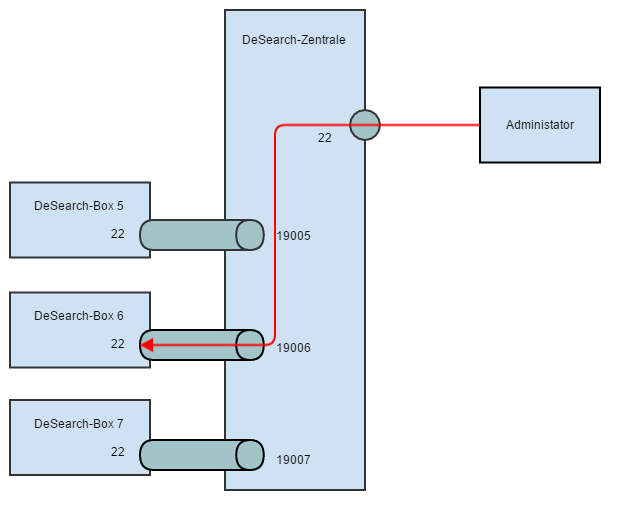
\includegraphics[width=\textwidth]{images/tunnel.png}
	\caption[Schematische Darstellung der Verwendung des SSH Tunnels]{\textbf{Schematische Darstellung der Verwendung des SSH Tunnels} - Beispielhaft ist hier eine Verbindung vom Administrator zur DeSearch-Box 6 dargestellt (roter Pfeil), Quelle: eigene Darstellung}
	\label{fig:tunnel}
\end{figure}

\newpage
\subsubsection{Installation einer neuen DeSearch-Box in der Testumgebung}\label{sssec:schritte}
Im Folgenden sollen alle Schritte erläutert werden, die für das Einbringen eines neuen Raspberry Pi als DeSearch-Box in das Testsystem durchgeführt werden müssen.
Voraussetzung dabei ist, dass der Pi bereits das Betriebssystem Raspbian vorinstalliert hat und mit einem WLAN- und Bluetooth-Dongle ausgestattet ist.\\
\textbf{Schritt 1: Internetverbindung}\\
Sofern noch nicht geschehen, muss der Raspberry mit dem Internet verbunden werden. Dies kann entweder schon im Testsystem geschehen, oder in der Entwicklungsumgebung in einem anderen Netzwerk. Der Zugriff auf den Raspberry erfolgt bei bereits bestehender Verbindung über SSH, andernfalls wird der Pi über HDMI an einen Monitor angeschlossen und zunächst direkt mit Maus und Tastatur konfiguriert. \\
\textbf{Schritt 2: Software aktualisieren}\\
Zunächst sollten einige unnötige Software-Installationen von Raspbian entfernt werden, da diese sonst bei jedem Update große Datenmengen herunterladen und installieren. Beispielsweise ist LibreOffice und WolframEngine vorinstalliert, wird aber auf der DeSearch-Box nicht benötigt. Mit \texttt{apt-get purge libreoffice* wolfram-engine} und \texttt{apt-get autoremove} werden diese deinstalliert und gelöscht. Anschließend wird die Software mittels \texttt{apt-get update} und \texttt{apt-get upgrade} auf den neuesten Stand gebracht. Hierfür muss der Pi eine Internet-Verbindung haben.\\
\textbf{Schritt 3: Hostname anpassen}\\
Um die DeSearch-Boxen später im Netz voneinander unterscheiden zu können, muss der Hostname des Gerätes angepasst werden. Hierfür wird der Hostname in der Datei \texttt{/etc/hostname} und in der Datei \texttt{/etc/hosts} von \texttt{raspberrypi} auf z.B. \texttt{pi9} geändert. Damit diese Änderung wirkt, muss der Pi neu gestartet werden.\\
\textbf{Schritt 4: Statische IP-Adresse konfigurieren}\\
Falls der Pi im WLAN noch nicht gefunden werden kann, ist die Alternative eine SSH-Verbindung über LAN. Damit diese funktioniert, wird eine statische IP-Adresse auf dem Interface eth0 konfiguriert. Dazu muss ein Eintrag in die Datei \texttt{/etc/network/interfaces} gemacht werden:\\
\texttt{auto eth0\\
	allow-hotplug eth0\\
	iface eth0 inet static\\
	address 192.42.42.2 // Dies ist die beispielhafte statische IP-Adresse\\
	netmask 255.255.255.0}\\
\textbf{Schritt 5: Netzwerkzugriff in der Testumgebung}\\
Je nach Vorgehensweise kann dieser Schritt auch bereits als erster Schritt erfolgen. Um die Zugangsdaten für das WLAN-Netzwerk der DHBW zu konfigurieren, muss die Datei \texttt{/etc/wpa\_supplicant/wpa\_supplicant.conf} bearbeitet werden. Hier wird der Eintrag (beispielhaft für das DHBW-Netzwerk) folgendermaßen angelegt:\\
\texttt{network=\{\\
	\tab ssid="DHBW-STUDENT"\\
	\tab key\_mgmt=WPA-EAP\\
	\tab identity="<Nutzername>"\\
	\tab password="<Passwort>"\\
	\}}\\
\textbf{Schritt 6: Tunnel zur Box einrichten}\\
Für den Zugriff auf die neue DeSearch-Box muss ein SSH-Tunnel von der Zentrale aus hergestellt werden(siehe auch Kapitel \ref{sssec:tunnel}). Hierfür wird im home-Verzeichnis zunächst die Datei \texttt{tunnel.sh} angelegt und mit folgendem Inhalt gefüllt:\\
\texttt{\#!/bin/bash\\
	/usr/bin/autossh -i /home/pi/tunnel -fN -R 19005:localhost:22 141.68.30.39}\\
Die Portnummer (hier 19005) muss für jeden Pi eindeutig sein.
Zudem wird die Datei \texttt{tunnel} im home-Verzeichnis erstellt, in der der Private Key des tunnel-Users auf der Zentrale abgelegt wird. Das Tunnel-Skript greift dann beim Aufbau des ssh-Tunnels auf diese Datei als Key zu. Nachdem diese beiden Dateien erstellt wurden, müssen die Berechtigungen angepasst werden. Mit \texttt{chmod 755 tunnel.sh} und \texttt{chmod 600 tunnel} wird das Skript ausführbar und nur der Pi-User hat Lesezugriff auf den Private Key. Als nächstes wird das tunnel-Skript in einen Cronjob eingefügt, damit der Tunnel immer selbständig aufgebaut wird, auch nach einem reboot des Systems. Hierfür ruft man \texttt{crontab -e} auf und fügt folgende Zeile ein: \texttt{@reboot /home/pi/tunnel.sh}\\
Als letzten Schritt sollte überprüft werden, ob das Tool autossh installiert ist. Andernfalls wird es mit \texttt{apt-get install autossh} installiert.\\
\textbf{Schritt 7: DeSearch-Software installieren}\\
Nachdem die Verbindung zu der Box und die Infrastruktur gesichert sind, kann nun die DeSearch-Software auf der Box installiert werden. Zunächst wird die Datei\\ \texttt{/etc/apt/sources.list.d/desearch.list} angelegt. In diese Datei fügt man folgende Zeile ein: \texttt{deb https://www.philipp1994.de/apt/ vivid desearch}. Somit wird festgelegt, aus welcher Quelle die DeSearch-Software bezogen wird. Der angegebene Server ist beispielhaft für das Testsystem und muss für die Produktivnutzung geändert werden. Anschließend wird mit \texttt{apt-get install apt-transport-https} die Installation über HTTPS ermöglicht. Dafür wird der Public Key des Quellservers benötigt, der mit\\ \texttt{wget https://philipp1994.de/philipp1994.de.gpg} heruntergeladen werden kann. \texttt{apt-key add philipp1994.de.gpg} installiert diesen Key, sodass die .gpg-Datei anschließend gelöscht werden kann. Ein Aufrufen von \texttt{apt-get update} lädt nun die verfügbaren Software-Updates für die DeSearch-Software herunter. Installiert wird die Software durch \texttt{apt-get install desearch-client}. Im Installationsprozess muss die Box-Nummer und die Service-URL angegeben werden (siehe Abbildungen \ref{fig:installation1} und \ref{fig:installation2}).
\begin{figure}
	\centering
	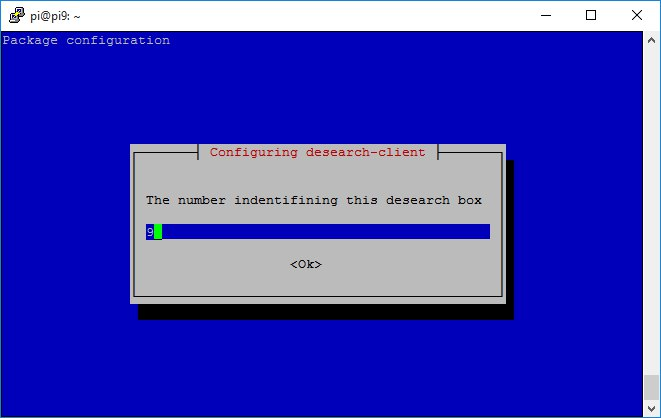
\includegraphics[width=\textwidth]{images/installation1}
	\caption[Eingabe der Box-Nummer bei Installation der DeSearch-Software]{Installationsprozess der DeSearch-Software, hier wird die Box-Nummer eingegeben. Quelle: eigene Darstellung}
	\label{fig:installation1}
\end{figure}
\begin{figure}
	\centering
	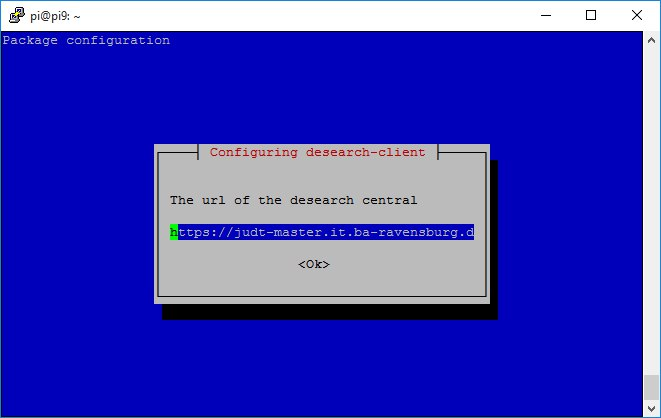
\includegraphics[width=\textwidth]{images/installation2}
	\caption[Eingabe der Service-URL bei Installation der DeSearch-Software]{Installationsprozess der DeSearch-Software, hier wird die Service-URL eingegeben. Quelle: eigene Darstellung}
	\label{fig:installation2}
\end{figure}  
Eine erfolgreiche Installation kann mit \texttt{service desearch-client status} überprüft werden. Hier sollte der Status \enquote{active(running)} angezeigt werden (siehe auch Abb. \ref{fig:systemctl-status}).\\
\textbf{Schritt 8: Bekanntmachen der Box an der Zentrale}\\
Im letzten Schritt müssen die neue DeSearch-Box und die Zentrale ihre Keys austauschen, um eine sichere Kommunikation zu ermöglichen (vgl. Kapitel \ref{cap:authentifizierung}). Hierfür muss das Python-Skript \texttt{/opt/desearch-client/keyExchange.py} ausgeführt werden. Gleichzeitig muss auf der Zentrale das Python-Skript \texttt{/opt/desearch-server/keyExchange.py} ausgeführt werden. So werden die Keys auf Server und Client generiert (dies kann auf einem Raspberry Pi einige Zeit dauern) und anschließend muss der User die Hash-Werte der Keys auf Zentrale und Box vergleichen. In Abbildung \ref{fig:keyEx} ist der Key-Exchange auf einer DeSearch-Box zu sehen. 
\begin{figure}
	\centering
	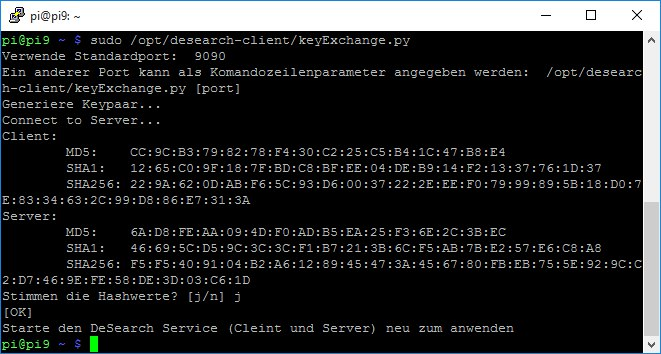
\includegraphics[width=\textwidth]{images/keyExchange}
	\caption[Key-Exchange zwischen DeSearch-Box und Zentrale]{Key-Exchange zwischen DeSearch-Box und Zentrale, hier wird der User aufgefordert, die Hash-Werte zu vergleichen. Quelle: eigene Darstellung}
	\label{fig:keyEx}
\end{figure}
Nach der Bestätigung ist die Box nun im System bekannt und kann sicher mit der Zentrale kommunizieren.

\nomenclature{LAN}{\textbf{L}ocal \textbf{A}rea \textbf{N}etwork}
\nomenclature{WLAN}{\textbf{W}ireless \textbf{LAN}}
\nomenclature{HTTP}{\textbf{H}yper\textbf{T}ext \textbf{T}ransfer \textbf{P}rotocol}
\nomenclature{HTTPS}{\textbf{H}yper\textbf{T}ext \textbf{T}ransfer \textbf{P}rotocol \textbf{S}ecure}
\nomenclature{ARM}{\textbf{A}dvanced \textbf{R}ISC \textbf{M}achines}
\nomenclature{RISC}{\textbf{R}educed \textbf{I}nstruction \textbf{S}et \textbf{C}omputer}
\nomenclature{CPU}{\textbf{C}entral \textbf{P}rocessing \textbf{U}nit}
\nomenclature{SD-Karte}{\textbf{S}ecure \textbf{D}igital Memory \textbf{Card}}
\nomenclature{URL}{\textbf{U}niform \textbf{R}esource \textbf{L}ocator}
\nomenclature{FTP}{\textbf{F}ile \textbf{T}ransfer \textbf{P}rotocol}
\nomenclature{SQL}{\textbf{S}tructured \textbf{Q}uery \textbf{L}anguage}
\nomenclature{ORM}{\textbf{o}bject \textbf{r}elational \textbf{m}apping}
\nomenclature{SSH}{\textbf{S}ecure \textbf{Sh}ell}
\nomenclature{GUI}{\textbf{G}raphical \textbf{U}ser \textbf{I}nterface}
\nomenclature{CA}{\textbf{C}ertificate \textbf{A}uthority}
\nomenclature{MITM Attake}{\textbf{M}an-\textbf{i}n-\textbf{t}he-\textbf{m}iddle Attacke}
	\section{Evaluierung der Lösungsergebnisse}
Die Lösungsergebnisse sollen im Folgenden Kapitel anhand fester Kriterien überprüft werden. Ein Kriterienkatalog wurde aus den Geschäfts- und Systemfällen entwickelt, die als Ergebnis aus einer studentischen Veranstaltung zu Projektbeginn entstanden sind (siehe Anhang \ref{anh:fälle}).
\subsection{Überprüfung der Erfüllungskriterien}\label{ssec:erfuellung}
Anhand der Kriterien in Tabelle \ref{tab:kriterien} soll die Problemlösung überprüft werden. Alle Kriterien werden in der Testumgebung an der DHBW Friedrichshafen durchgespielt und anschließend bewertet.
\begin{table}[h]
\begin{tabular}{ | p{2,5cm} | p{5cm} | p{5cm} | p{2,5cm} |}
	 \hline
	 \textbf{Kriterium} & \textbf{Beschreibung} & \textbf{Erwartetes Ergebnis} & \textbf{Erfüllungs-grad} \\ \hline
	 Vermisster Patient wird erfasst & Ein Patient wurde in der Zentrale als vermisst markiert und die entsprechende Marke befindet sich in Reichweite einer DeSearch-Box & Die Box erkennt die entsprechende Marke und meldet sich bei der Zentrale & tbd \\ \hline
	 Andere Marken werden ignoriert & Ein Patient wurde in der Zentrale als vermisst markiert und Marken von anderen Patienten befinden sich in Reichweite einer DeSearch-Box & Die Box erkennt, dass die Marken in Reichweite nicht vermisst werden und meldet nichts zurück & tbd \\ \hline
	 DeSearch-Box wird konfiguriert & Eine neue DeSearch-Box soll konfiguriert bzw. eine bestehende Box soll angepasst werden & Konfigurierte und im System verbundene DeSearch-Box & erfüllt; Siehe Kapitel \ref{sssec:schritte} \\ \hline
	 DeSearch-Box wird befestigt & Eine DeSearch-Box soll am Einsatzort befestigt werden & Vor Vandalismus und Diebstahl gesicherte, im Netzwerk erreichbare Box mit permanenter Stromversorgung & nicht zutreffend für Prototyp, Anforderung an Produktivsystem \\ \hline
	 temporärer Ausfall DeSearch-Box & Ein unerwarteter Ausfall der Box tritt zeitweise auf & Nach Reboot der Box soll sich diese selbständig wieder im System anmelden und den Scan-Vorgang wieder aufnehmen & erfüllt durch Services und cronjob, siehe Kapitel \ref{sssec:services}\\ \hline
	 permanenter Ausfall DeSearch-Box & Ein unerwarteter Ausfall der Box tritt permanent auf, die Box sendet keine alive-Meldungen mehr & Das System muss den Ausfall feststellen, sodass die Box manuell wieder im System reaktiviert werden kann & tbd \\ \hline
	 DeSearch-Box fordert gesucht-Liste an & Die Box fordert periodisch die aktuelle Liste der gesuchten Marken bei der Zentrale an & Die Zentrale übermittelt der Box die aktuelle Liste der gesuchten Marken & erfüllt, Anfrage alle 10 Sekunden \\ \hline
	 App fordert gesucht-Liste an & Die Benutzeroberfläche fordert beim Start der Applikation die aktuelle Liste der gesuchten Personen an & Die Zentrale übermittelt der App die aktuelle Liste der gesuchten Personen & erfüllt, siehe Kapitel \ref{sssec:ui}\\ \hline
	 Mitarbeiter deaktiviert Marke & Eine gesuchte Marke wurde gefunden, aber die gesuchte Person trägt dieses Kleidungsstück momentan nicht & In der App wird die Marke deaktiviert, die Zentrale entfernt die Marke von der gesucht-Liste & tbd \\ \hline
	 Person wurde gefunden & Ein Mitarbeiter beendet die Personensuche in der App & Die Zentrale entfernt alle entsprechenden Marken von der gesucht-Liste & erfüllt, siehe Kapitel \ref{sssec:ui}\\ \hline
	 
	
\end{tabular}
\caption{Erfüllungskriterien zur Überprüfung der Problemlösung}
\label{tab:kriterien}

\end{table}
\subsection{Zuverlässigkeit der Infrastruktur}
Für die Zuverlässigkeit der Infrastruktur wurden zahlreiche Schritte unternommen, die das System ausfallresisent machen. %TODO aufzählen

	\section{Schlussteil}
\subsection{Zusammenfassung}
\subsection{Ausblick}

	
	
	% Abschluss
	\bibliography{literatur/Studienarbeit_literatur}
\newpage

	%\renewcommand{\indexname}{Stichwortverzeichnis}
\printindex
\newpage

		
	% Anhang
	\renewcommand{\thetable}{\Alph{section}.\arabic{table}}              % Tabellennummerierung mit Section
	\renewcommand{\thefigure}{\Alph{section}.\arabic{figure}}            % Abbildungsnummerierung mit Section
	\renewcommand{\thelstlisting}{\Alph{section}.\arabic{lstlisting}}    % Listingsnummerierung mit Section
	
	\begin{appendix}
	
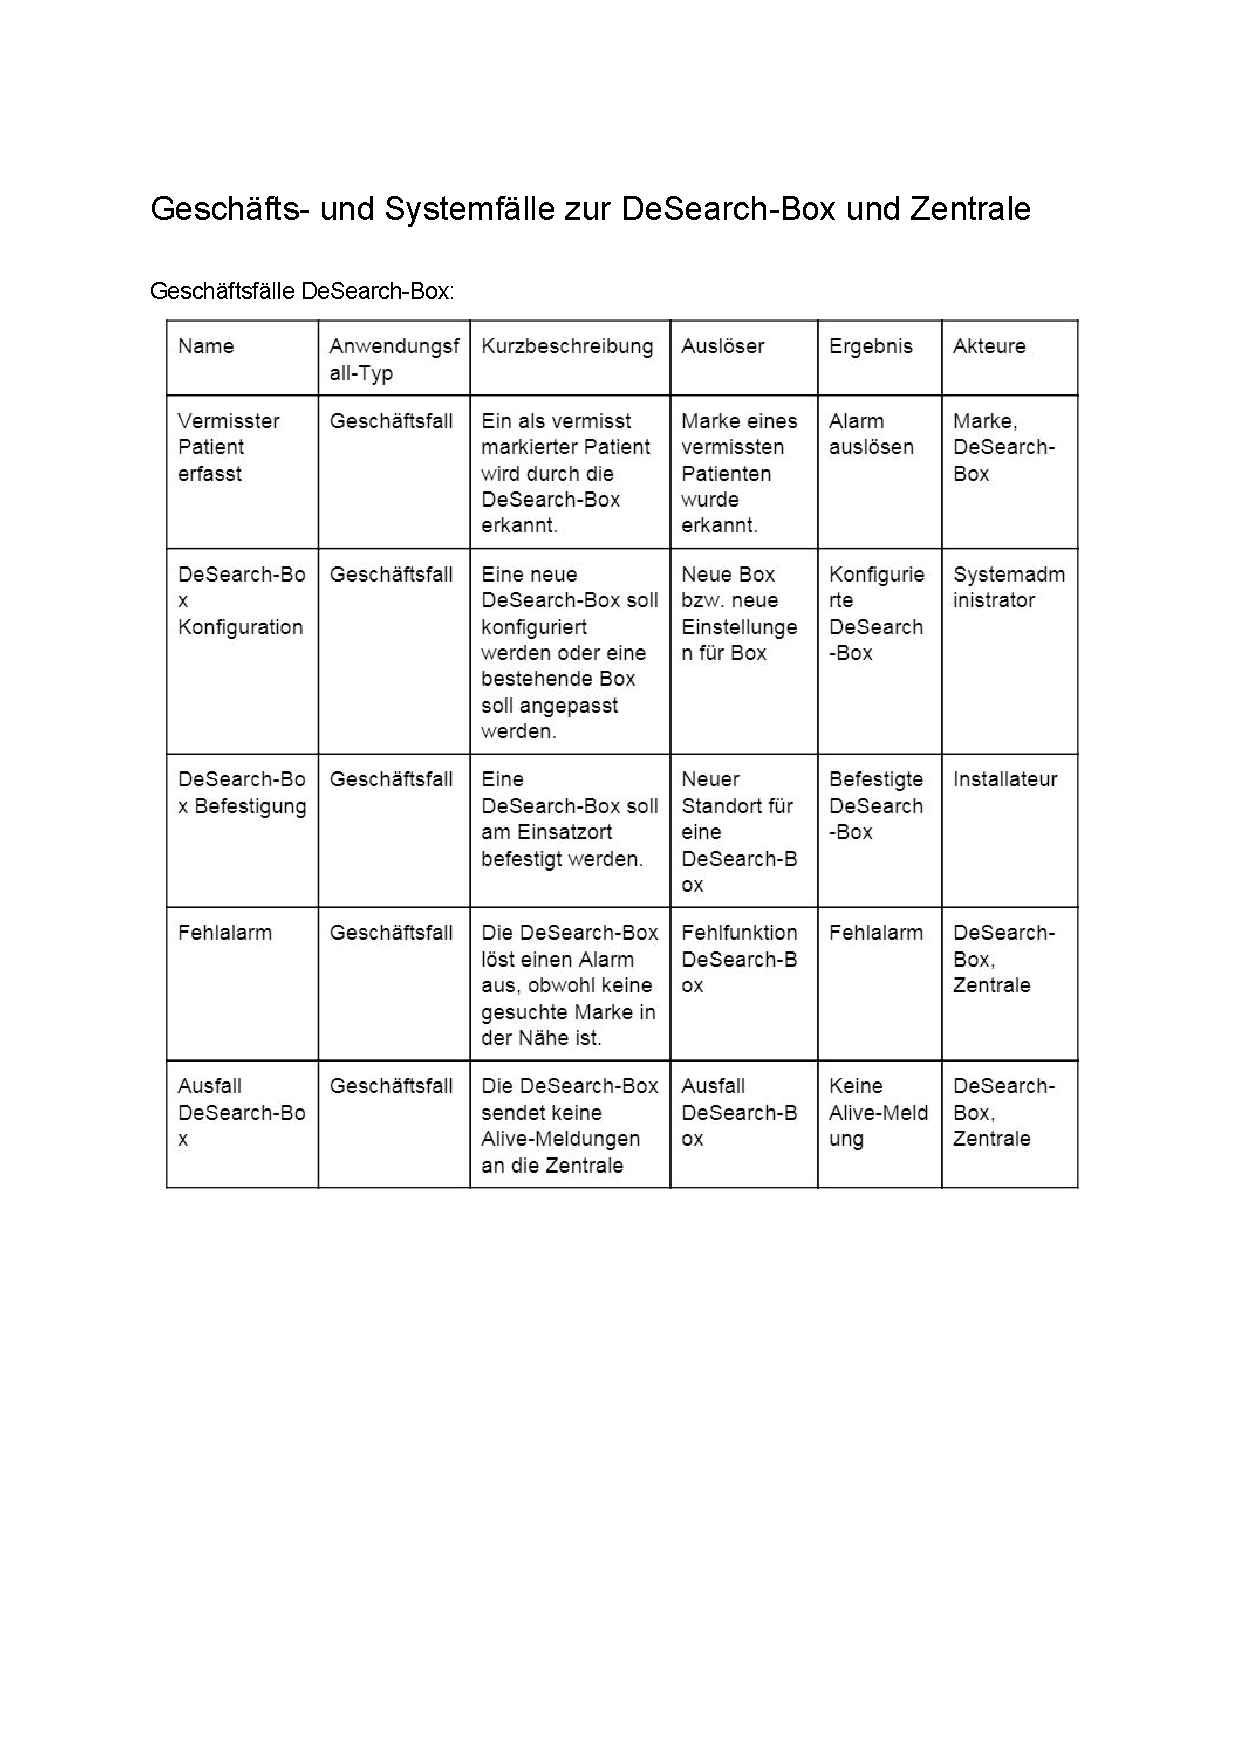
\includepdf[pages=1,scale=0.8,clip,pagecommand={\section{Geschäfts- und Systemfälle zur Überprüfung der Ergebnisse}\label{anh:fälle}}]{src/Geschaefts-Systemfaelle.pdf}

\includepdf[pages=2-,scale=0.9,clip,pagecommand={}]{src/Geschaefts-Systemfaelle.pdf}
\newpage
%\section{Master-Detail-Layout}\label{anh:master-detail}

	\end{appendix}
	
	
\end{document}

%%%%%%%%%%%%%%%%%%%%%%%%%%%%%%%%%%%%%%%%%%%%%%%%%%%%%%%%%%%%%%%%%%%%%%%%%%%%%
%%                                                                         %%
%% /\   /\         Ab hier keine Änderungen mehr vornehmen         /\   /\ %%
%%                                                                         %%
%%%%%%%%%%%%%%%%%%%%%%%%%%%%%%%%%%%%%%%%%%%%%%%%%%%%%%%%%%%%%%%%%%%%%%%%%%%%%